\chapter[Passwords -- A User Perspective]{Passwords -- \\
	A User Perspective}\label{chap:rw:user_perspective}
%lingo: arduous

``but his thoughts were so full of the great riches he should possess, that he could not think of the word to make it open, but instead of `Sesame,' said, `Open, Barley!' and was much amazed to find that the door remained fast shut. He named several sorts of grain, but still the door would not open, and the more he endeavoured to remember the word `Simsim,' the more his memory was confounded, and he had as much forgotten it as if he had never heard it mentioned.'' (Kasim's predicament in \textit{Ali Baba and the Forty Thieves}) \todo{this could be the opening of the chapter / fancychapter}

%alternatively: this: [King Roland has given in to Dark Helmet's threats, and is telling him the combination to the "air shield"] Roland : One. Dark Helmet : One. Colonel Sandurz : One. 
% Roland : Two. Dark Helmet : Two. Colonel Sandurz : Two.
%Roland : Three.
%Dark Helmet : Three.
%Colonel Sandurz : Three.
%Roland : Four.
%Dark Helmet : Four.
%Colonel Sandurz : Four.
%Roland : Five.
%Dark Helmet : Five.
%Colonel Sandurz : Five.
%Dark Helmet : So the combination is... one, two, three, four, five? That's the stupidest combination I've ever heard in my life! That's the kind of thing an idiot would have on his luggage!

Morris and Thompson were already concerned with user behavior regarding passwords in 1979 \cite{Morris1979PasswordSecurity}. They identified that users choose predictable passwords and that this can be leveraged for attacks. So, they suggested enforcing a certain minimum password length (six characters). At the time, the users were mostly professionals that received training to operate computers and could thus also have been trained to pick less predictable passwords \cite{Maguire2012YouOnlyLiveTwice}. But as computers were introduced to a larger audience, more people were exposed to password authentication. Naturally, this also induced a growing number of attacks, and it is increasingly difficult for users to defend themselves against them (see. Section \ref{sec:rw:attack_vectors}). Nowadays, password policies are in place that require not only a minimum of eight characters, but also mandate mixed-case letters, digits and special symbols to start with. The HCI community noticed the users' struggle in the 1990s and that we can -- and should -- design authentication systems with usability in mind. Perhaps, one of the breaking points where a new school of thought turned up in the literature was a paper by Adams and Sasse in 1999 \cite{Adams1999UsersEnemy}. The central and novel theme in there was a shift from \textit{fixing} the user to \textit{acknowledging} user behavior and designing for it. The paper managed to see over 1500 citations as of writing this.

This chapter looks at the literature that mostly came after this seminal work. It discusses the users' problems, solutions, feelings, and opinions about using passwords. An essential goal is to give the reader an empathetic perspective and provide background information to understand why it seems hard to come up with viable solutions to make users' lives less frustrating. To get there, we first take a brief look at conducting user research with passwords. Hereafter we disseminate typical coping strategies and solutions. The chapter concludes with a comment on the discourse that has been going on between the very different schools of thought about passwords. 

%Each person who gets in contact with the Internet will at some point create a password.

% Everyone develops their own strategy how to do this and how to cope with passwords, probably already in early teenage years \cite{VonZezschwitz2013SurvivalShortest}. These strategies however are not unique and show macroscopic commonalities, which became evident after the first large-scale password leaks. 

%Important: Under coping strategy, we also understand the selection process, because choosing a weak password over a strong one is also one way to \textit{cope} with the large number of passwords and the memorability burden. (make sure to mention this in the general introduction already.)

\section{Methodology: Running Password Studies}\label{sec:rw:methodology}
% not relevant: how to measure password strength. solely focus on the ``HOW'' of data collection
Before we report on insights about user behavior regarding passwords, we take a look into running studies that focus on passwords. There are two central aspects that make collecting data particularly challenging: acting ethically and maintaining high ecological validity of the data. In fact, these two goals create an area of tension that demands a critical selection of methods. Komanduri \etal note that ``ideally, password studies would be conducted by collecting data on real passwords created by real users of a deployed system'' \cite{Komanduri2011OfPasswordsAndPeople}. But this would mean that researchers obtain access to the user accounts that were under investigation. This is ethically questionable \cite{Egelman2012ItsNotStealing}. Maybe the researchers themselves are benevolent, but the data is precious and thus could bring attackers to the scene. Since absolute security can barely be guaranteed, it is best to avoid that users disclose their actual credentials during a user study to the researchers.

\subsection{General Considerations for User Studies as Data Source}
If we cannot collect the users' real password in its original form, what is the best way to measure, e.g., cause and effect of novel interventions? There are several alternatives. 
% first solution: have people create a new one. 
\subsubsection{Password Creation Tasks} First, one asks participants to create a new password during the user study and stores these passwords as part of the dataset. This approach resolves the issue of real-world password disclosure, but introduces a number of problems.
% ethical dilemma #1: do people know that their passwords are studied? 
Studies should be ethical and thus transparent for the most part. Hence, the study topic should be known to the participants. However, if participants know that their passwords are studied, this could induce protective reactions to prevent giving hints about their real passwords at all. In that case, the participants' selection strategy does not resemble much to their real-world behavior and thus the ecological validity of the data is low \cite{Shay2012CorrectHorseBatteryStaple}. 
% give a realistic risk
Although it appears trivial, Fahl \etal suggest that in this scenario, asking the participants whether they had acted like they normally would is a suitable indicator that helps in weighting the data \cite{Fahl2013EcologicalValidityPasswordStudy}. It is also recommendable to give users a specific scenario that allows them to immerse themselves in the task. Komanduri \etal argue that having participants create passwords for fictional email accounts leads to more authentic behavior \cite{Komanduri2011OfPasswordsAndPeople}.
% ethical dilemma #2: sharing the collected data. 
Some users, however, are less protective and provide one of their real passwords regardless of the instruction (e.g. 26.5\% in Fahl \etal's study \cite{Fahl2013EcologicalValidityPasswordStudy}). The result is the same as if the purpose of the study was concealed through an act of deception, which is occasionally done in psychology studies (for a discussion see \cite{Tai2012Deception}). For example, it can suffice to tell participants a convincing \textit{cover story}, e.g. that the purpose of the study is to do a usability test of a social networking site, which also happens to involve an account setup process (see \cite{Furnell2017GuidanceCompliance}). The data would be ecologically valid because it removes observer-expectancy and other biases. For the researchers, however, it is extremely difficult to tell ``real'' passwords and ``new'' passwords apart. Thus, phishing or man in the middle attacks are sometimes carried out. Haque \etal conducted a laboratory study where they told participants a cover story to create new accounts for popular websites \cite{Haque2014Hierarchy}. The websites, however, were re-created by the researchers and stored the passwords on their own servers instead of performing actual registrations. Egelman \etal used a proxy server to intercept traffic between the users and a real online portal \cite{Egelman2013DoesMyPasswordGoUpToEleven}. They also altered the websites to communicate their cover story that the password had expired. This, however, creates an ethical conundrum, if the dataset is published along with the paper. To allow others to verify that research is valid, reliable, and generalizable, a published dataset is desirable, but in Egelman \etal or Haque \etal's study this would put real user accounts at risk.
% ethical dilemma #3: sharing cracking algorithms.
Much in the same vein, sharing research about successfully attacking passwords produces a similar dilemma. For instance, one can put forward new cracking approaches (e.g. \cite{Marechal2008AdvancesPWCracking, Narayanan2005FastDictionaryAttacks, Schmidt2013Pitfalls, Weir2009PCFG}) that potentially affect common strength metrics (see Section \ref{sec:rw:pw_strength_metrics}) -- but attackers also benefit from this kind of knowledge. From an HCI perspective, one can also unfold how users select passwords, which allows optimizing cracking efficiency \cite{Weir2010MetricsPolicies, Wheeler2016zxcvbn}. 


% SOLUTIONS TO ETHICAL PROBLEMS
There are several methods to avoid acting unethically in studies where users are required to create passwords. 
% IRBs
First of all, studies involving human subjects are assessed by an \gls{IRB}, especially in the United States. This is done to ensure an ethical study design that is unlikely to cause participants any harm. The \gls{IRB} might mandate a thorough debriefing of participants and meticulous documentation of the experiment. In Europe, however, password studies are less commonly evaluated by an IRB (or authors fail to mention the process in their papers) \ar. 
% Do not publish data sets.
Secondly, one can refrain from releasing the data set, even if user names are removed. In fact, almost all publications on passwords collected during a user study omit publishing the corresponding data set. Only the abstract analysis is published and this is a widely-accepted standard practice, despite the questionable reliability. 
% Differential privacy.
A rather novel approach that reduces the likelihood of made-up data relies on the idea of publishing differentially private data sets. Here, algorithmically generated noise, which is indistinguishable from the orignal data, is added to the data set to preserve privacy of users. For password frequency lists, passwords could be mangled and extended by generated passwords that resemble real ones. Adversaries lack information whether the data is usable as signal or noise.
This way, Blocki \etal managed to release a private frequency list of passwords at Yahoo that Bonneau had already anonymously analyzed in \cite{Bonneau2012ScienceOfGuessing}. 
% Encryption
Moreover, instead of collecting newly generated passwords in plain text, it is possible to store a hashed version. For instance, Wash \etal had participants install a browser extension that logged all form submits that included a password field \cite{Wash2016UnderstandingPasswordChoices}. To study reused passwords, they hashed and sent them over a secure connection to their servers. As long as a slow hash function and a strong salt are used, this approach is uncritical. However, it merely allows observing if the hashes match on several sites.
% Meta data
Finally, as a last option to collect password data, researchers can log meta-data instead of passwords. For instance, Von Zezschwitz \etal used a ``meta password'' that described the participants' actual passwords \cite{VonZezschwitz2013SurvivalShortest}, but which was insufficient to reconstruct the original. This can include the number of characters, upper-/lowercase letters, digits, and even proactive strength estimations. To collect the data, participants in von Zezschwitz \etal's study were provided with an offline password analysis tool. They entered their password into that and copy-pasted the result of the analysis into the questionnaire form. If one does not want to examine the passwords qualities, this approach is absolutely feasible. Florêncio and Herley used a similar approach for the large-scale data collection with around 500000 participants to avoid running into privacy issues \cite{Florencio2007LargeScaleStudyPasswordHabits}. The information transmitted to the logging server was pseudonymized and contained only meta features. The only downside is that one cannot run further analyses on the passwords, e.g. if a new strength metric is considered.

% second solution: SELF REPORT instead of the task to create a password
\subsubsection{Retrospective Self Report}
If one wants to refrain from having users create a new password, one can study their past behavior in different ways. In its simplest form, participants are simply asked to describe how they create passwords. Stobert \& Biddle did this in extensively to create the Password Life Cycle model \cite{Stobert2014PasswordLifeCycle} (see Section \ref{sec:rw:user-behavior}). Ur \etal used interviews to find out what users do to make their passwords stronger \cite{Ur2015PWCreationLab}. Das \etal found out through retrospective interviews that social contacts have a strong impact on users' security decisions \cite{Das2014EffectSocialInfluenceSecuritySensitivity}. Most commonly, however, typical online surveys feature a number of questions about personal behavior and attitudes, e.g. \cite{Adams1997MakingPWsSecureAndUsable, Gaw2006PasswordManagement, Kuo2006HumanSelectionMnemonic,Riley2006WhatUsersKnowWhatTheyDo, Shay2010EncounteringPasswordRequirements}. Questions about passwords are easy to implement in a survey and respondents can always choose how much they want to share. However, one has to stay aware that social desirability lowers the reliability of the data: since the media also to their part in shaming users for picking ``bad'' passwords, people may respond dishonestly about their password behavior. Many people are uncomfortable admitting their password is as simple as 12345. Another problem results from fading memories. Since most users have more than one password, it might be difficult for them to recall the correct past behavior. However, not only password studies suffer from this bias, but any study involving self report in general. 

\subsubsection{Principles}\label{sec:rw:principles-experiments}
From user research in \acrshort{USEC} of the past decades, Krol \etal derive a set of general principles that researchers ought to consider when conducting experiments in security and privacy \cite{Krol2016ExperimentDesign}. We can integrate password studies in there:
%\vspace*{-0.5cm}
\paragraph{Primary Task} Creating a password should not be the sole task in the study. Instead, participants should achieve a primary task by authenticating with passwords, e.g. using a new system for a period of time \cite{Brostoff2000PassfacesEvaluation}. The reasoning behind this principle is that security tasks are secondary tasks and this constraint needs to be reflected in the experiment. However, re-focusing on a separate primary task is not always possible, e.g. in surveys. 
\vspace*{-0.5cm}
\paragraph{Realistic Risk} Users should be able to realistically estimate the risk for secure interactions. As mentioned above, Komanduri \etal suggest carefully selecting real-world scenarios to achieve this \cite{Komanduri2011OfPasswordsAndPeople}.
\vspace*{-0.5cm}
\paragraph{No Priming} Whenever human behavior is studied, experiments should avoid influencing and biasing participants with certain information. This avoids unnatural behavior.  
\vspace*{-0.5cm}
\paragraph{Double Blind Experiments} If possible, the person carrying out the actual experiment should be involved in the planning and design of the study. Moreover, the participants should not know the details of the study, either. On the experimenter side, unconscious bias and influence is mitigated, and participants also do not know the ``treatment'' they receive (if any). Although this is a desirable goal, there is little evidence that experiments are usually carried out in this way. 
\vspace*{-0.5cm}
\paragraph{Context Definition} To increase internal validity, it is necessary to define the terms \textit{threat model}, \textit{security}, \textit{privacy}, \textit{usability}, depending on which are relevant for the study. A precise definition avoids misunderstanding and improves transparency, credibility, and trustworthiness of the experiment.\\ 

\noindent These principles can serve as a rough quality assessment of presented research, although in many instances, not all principles will be fully addressed.

% briefly show the benefits and drawbacks of each method. 
%TODO maybe some Usable Security book already has this? look into garfinkel/cranor book...
\subsection{Analyzing Password Leaks and (Semi-)Public Data}
% frequency lists are a source of data
Instead of users creating new passwords, it is possible to make inferences about their behavior from already existing data (for an overview see Table \ref{tab:rw:password_leaks}). Password frequency lists are readily available on the Internet \footnote{An example repository containing a wide range of leaked passwords is available under \url{https://github.com/danielmiessler/SecLists/tree/master/Passwords} \la{09.01.2018}}. The sources can often be traced back to illegal attacks, which makes the use of such data somewhat questionable. However, it is a widely accepted method to contrast real-world and study behavior. The data set that has probably been studied the most originates from a breach at RockYou, a software development firm specialized at games for social networks. In 2009, an attacker used an SQL injection to download around 32 Million plain-text passwords. For instance, Veras \etal visualized semantic properties of passwords in this dataset and highlight the high occurrence of dates in there \cite{Veras2012VisualizingSemanticsPasswords}. Wheeler relied on it to build the zxcvbn password strength estimation system. More often, though, these data sets serve as training data for password guessability benchmarks. Weir \etal took the RockYou passwords to train their \gls{PCFG} which served as a demonstration that entropy is not a feasible strength metric for user-chosen passwords. Afterwards, it was integrated into the training set of \gls{PGS}. \gls{PGS} is mostly used to gauge passwords collected through a user study, e.g. under different policies \cite{Shay2016DesigningPasswordPolicies} or interventions \cite{Ur2017DataDrivenPWMeter}. In conclusion, publicly leaked data sets can often serve as ground truth for studies that aim to provide new insights.  

%
% PASSWORD LEAKS, label: tab:rw:password_leaks
% password leaks

% Table generated by Excel2LaTeX from sheet 'leaked datasets'
\begin{table}[htbp]
  \centering
  \caption{\label{tab:rw:password_leaks} Example password leaks of the past five years. Some of the data served security researchers to analyze user behavior and create more effective strength estimation algorithms.}
    \begin{tabular}{lrrl}
    \textbf{Data Source} & \textbf{\# PWs} & \multicolumn{1}{l}{\textbf{Year}} & \multicolumn{1}{l}{\textbf{Literature}} \\
    \midrule
    \midrule
    RockYou & 32 M  & 2009  & \todo{add references that used the data.} \\
    LinkedIn & 164 M & 2016  & \todo{provide references for the info in this table} \\
    Dropbox & 68 M  & 2012  &  \\
    MySpace & 360 M & 2013  &  \\
    ebay  & 145 M & 2014  &  \\
    Adobe & 36 M  & 2013  &  \\
    Yahoo & 1 B   & 2013  &  \\
    \end{tabular}%
\end{table}%

% https://pgs.ece.cmu.edu/ at the bottom has a couple of statistics what kind of data they use.
% DeCarnedeCarnavalet2015PasswordMeters too

%
%

\subsection{User Study Methods in Password Research}
Research in \acrshort{USEC} takes advantage of the toolbelt of \acrshort{HCI} research in general. In the following, the most common methods for password studies are portrayed.
\paragraph{Laboratory studies}
% not focused on password: \cite{Sotirakopoulos2011ReplicationSSLWarnings}
To gain the greatest control over experimental parameters, laboratory studies are the go-to method. Both qualitative and quantitative studies are carried out in the lab, with a slight surplus of qualitative studies. Among the most common methods, one finds (semi-)structured interviews (\cite{Adams1997MakingPWsSecureAndUsable,Gaw2006PasswordManagement, Stobert2014PasswordLifeCycle, Ur2015PWCreationLab, Weirich2001PrettyGoodPersuasion}) and usability testing (\cite{Egelman2013DoesMyPasswordGoUpToEleven,Forget2007HelpingUsers,Forget2015CYOA,Gross2016CognitiveDepletion,Imran2015PWsAdultsChildren, McCarney2012Tapas,Mcevoy2016ContextualizingMnemonicPhrase,Ruoti2015AuthenticationMelee, Yang2014EntryAffectsPasswordSecurity,VonZezschwitz2014HoneyIShrunkTheKeys}). Password memorability can be studied in the lab (\cite{Egelman2013DoesMyPasswordGoUpToEleven,Fahl2013EcologicalValidityPasswordStudy,Forget2008MemorabilityPersuasivePasswords,Mcevoy2016ContextualizingMnemonicPhrase,Yan2004PasswordMemorabilitySecurity}). Studying short-term recall usually follows a mental-rotation task (e.g. \cite{Kraus2017Emoji,Yang2014EntryAffectsPasswordSecurity}). Long-term memorability studies in the lab are less common, because they require participants to return to the lab, which may be too bothersome for many. For alternative authentication schemes, this may, however, be the only option. 

Although technically it is not a ``lab'' environment, café studies sometimes are closely related to lab studies. Von Zezschwitz \etal collected qualitative and quantitative data on participants' past password behavior by inviting customers in a café to join them for a free coffee \cite{VonZezschwitz2013SurvivalShortest}. The experimenter has almost as much control as in a lab to answer certain research questions. Only the surroundings may distract somewhat. Other methods like participatory design / co-creation (\cite{Coventry2014SCENEBehavioralNudges,Read2009UnderMyPillow}) and focus groups (\cite{Eargle2015YouCanDoBetter,Hang2015Dissertation,Harbach2016HardLockLife,Singh2007PasswordSharing}) are possible, but less frequently reported than interviews and usability tests. A common drawback of lab studies lies in the high costs, time consumption to carry them out, smaller sample sizes, and reduced ecological validity.

\paragraph{Field-Studies}
Field studies for password research come in many flavors. 
% regular online surveys (no mTurk)
\textbf{Online surveys} are among the most common methods used in the field (\cite{Gaw2005ReuseRecycle,Halevi2013PilotStudyPersonality,Haque2014Hierarchy,Huh2017TooBusy, Kuo2006HumanSelectionMnemonic,Mazurek2013Measuring,Riley2006WhatUsersKnowWhatTheyDo, Violettas2014PasswordsAvoidGreece}), due to their lower cost and comparatively easy implementation. Other advantages like increased sample size and more diversity in the data speak in favor of online surveys. Survey tools like surveymonkey.com come in handy, but usually lack seamless integration of interactive prototypes. If a prototype should be evaluated through a survey, however, one has to either implement the entire survey structure or redirect participants from the survey platform to the prototype and back. Surveys are also the weapon of choice if there is an opportune moment that is worth studying. Mazurek \etal took the opportunity to distribute online questionnaires after a new password policy was introduced at \acrshort{CMU} \cite{Mazurek2013Measuring}. Fahl \etal profited from a similar situation at Leibniz-University Hannover, and Renaud \etal could even distribute surveys on the same topic across multiple years in this way \cite{Renaud2017LessonsLearnedNudges}. Interestingly, there does not seem to be a special, standardized survey construct to measure the usability, respectively user experience, of password systems. Other \gls{HCI} sub-fields more frequently use, for example, the NASA-TLX, \gls{PANAS} or AttrakDiff constructs to establish comparability with other studies. Notable exceptions were reported by Kraus \etal, who used AttrakDiff to evaluate emoji-based authentication \cite{Kraus2017Emoji}. The NASA-TLX was used by Fraune \etal, \cite{Fraune2013UserCreatedPictures}, Sherman \etal \cite{Sherman2014UserGeneratedGesturesAuth}, and Yang \etal \cite{Yang2014EntryAffectsPasswordSecurity}. Lately, the \gls{SeBIS} gains more attention, because it serves as a self-assessment that can help the interpretation of actions taken during a user study  \cite{Egelman2015SeBIS, Egelman2016BehaviorEverFollows, Wash2016UnderstandingPasswordChoices,Wash2017SelfReport}.

% mTurk studies
A special kind of online studies that has been extensively used and propagated by \acrshort{CMU} researchers leverage \textbf{crowd-sourcing} platforms like the Amazon Mechanical Turk (\gls{mTurk})\footurl{https://www.mturk.com/}{10.01.2018}. Survey respondents are recruited by paying each one a small amount of money for a valid response. This way, increasing the sample size is straight-forward, if many users have already signed up on the platform and are eligible for the \acrfull{HIT}. Workers (known as ``turkers'') form an increasingly diverse population \cite{Ross2010WhoAreTurkers}, which is another benefit.
% mturk examples.
In password research, for instance, Kelley \etal's high-impact work on password guessability collected around 12000 passwords using \gls{mTurk} \cite{Kelley20012GuessAgain}. Ur \etal had participants rate the strength and memorability of a given set of passwords, which allowed them to identify certain misconceptions \cite{Ur2016PerceptionsPassword}. Mazurek \etal compared features of passwords created by turkers to real passwords of students and staff at their university \cite{Mazurek2013Measuring}. They take the large similarities of the two data sets as evidence that passwords created during an mTurk study are a reliable and valid data source, so there is no urgent need to analyze passwords of a deployed system. Shay wrote a PhD thesis specifically about evaluating password policies with crowd-sourced data \cite{Shay2015UsablePoliciesMTurk}. 
% slightly starting to address issues
In many cases, e.g. \cite{Shay2014CanLongPasswordsBeSecureAndUsable,Shay2016DesigningPasswordPolicies,Ur2017DataDrivenPWMeter}, the primary task is to create a fictional account or merely a password under certain constraints, which apparently violates Krol \etal's study principles \cite{Krol2016ExperimentDesign}. It is especially interesting that most studies are announced as some kind of password study, probably mandated by \glspl{IRB} . But Mazurek \etal's work demonstrates that this limitation is bearable. Moreover, studying the long-term memorability of passwords is facilitated, because participants can be invited to return through an internal, anonymous messaging system. It is also possible to create more complex study designs with mTurk, e.g. if multiple device types should be used by the turkers to create passwords \cite{Melicher2016UsabilityMobileTextPasswords}. 
% issues with mTurk studies
Despite the wide range of advantages, there are shortcomings of crowd-sourced approaches as with any study method. First, turkers are incentivized to complete as many HITs as possible on the platform to earn money. Thus, completing a survey by providing quick answers without reading the questions could lead to unreliable data. Instructional Manipulation Checks (IMCs) and attention check questions (ACQs) can mitigate this problem \cite{Oppenheimer2009InstructionalManipulationChecks, Peer2017BeyondTheTurk}. Turkers are only paid if the commissioner accepts the HIT as valid, thus IMCs and attention checks are useful indicators here. Moreover, as of now, the mTurk platform can only be used in certain countries, e.g. the USA or UK. European alternatives exist, but are not yet par in terms of user base, response times, and feature set \cite{Peer2017BeyondTheTurk}. 

% diary studies
Aside from surveys, \textbf{diary studies} about passwords have proven feasible in the past. Inglesant and Sasse found out through a diary study that employees struggle with frequent password changes, which might not have become evident using other study means \cite{Inglesant2010TrueCostOfUnusablePolicies}. Hayashi and Hong used this method to analyze password re-use across different computers, services, and organizations \cite{Hayashi2011DiaryStudyPWs}. Since password authentication is a secondary task, keeping a diary of authentication events helps participants provide reliable behavioral data. However, it requires much effort to continuously stay aware of one's actions to log them. To avoid that participants forget logging and other self-reporting bias \cite{Wash2017SelfReport}, it can be worthwhile to ask them small questions in situ. This method, known as \textbf{\gls{ESM}}, requests short responses either in predefined intervals or when the system detects a relevant event. ESM has not seen much attention in password studies on the web (Lyastani \etal provide one exception \cite{Lyastani2017ImpactPWMPasswordStrength}), but mobile authentication has been studied with this method \cite{Harbach2016HardLockLife}. Users carry their personal mobile with them almost all the time, so there is a high chance of successfully receiving the experience sample. ESM was also found useful for studies about security warnings in browsers \cite{Akhawe2013AliceInWarningland,Felt2016RethinkingConnectionSecurityIndicators}.

% automated logging
Perhaps, ESM is underused for password studies, because it is possible to automatically detect such events and survey the participants before and/or after the \textbf{automatic data collection}. Florêncio and Herley conducted one of the largest studies to date on password habits with this method \cite{Florencio2007LargeScaleStudyPasswordHabits}. Their intention was to find out among other things A) how often people type passwords, B) how many sites share a password C) how many distinct passwords a user has, and D) how the strong the passwords are. Working at Microsoft, they were granted to utilize the Windows Live Toolbar for Internet Explorer to collect in-the-wild data from up to 500,000 users during three months of running the collection. They conceived the method of protected password lists (PPL) to avoid intruding into people's privacy -- a kind of meta description of passwords which is sent to the logging server instead of the original password. It was thus not possible to trace the incoming data back to a specific user. However, there are a number of limitations this method. The authors point out that the anonymity of the incoming data-stream might have resulted in over-counting of entries. Also, it was not measured how long the actual password entries takes. If users only used regular dictionary words without any modification as their passwords, the key logging module of the toolbar would have recorded a password reuse event (PRE) every time the user entered that word -- also in regular online communication. Nevertheless, the fact that users are typically focused on their primary tasks, background logging helps to collect unbiased data with high ecological validity. 

% deployed systems
A final option to study passwords in the field is to collect and analyze them in an already deployed system (\textbf{in-situ evaluation}), which would be the ideal data source, according to Komanduri \etal \cite{Komanduri2011OfPasswordsAndPeople}. Brostoff and Sasse utilized a coursework system to evaluate Passfaces as alternative to passwords \cite{Brostoff2000PassfacesEvaluation}. Similarly, Renaud \etal used a coursework tool to evaluate the effectiveness of different password nudges \cite{Renaud2017LessonsLearnedNudges}. Mazurek \etal gained access to passwords of their University's \gls{SSO} and were able to break down differences in password selection behavior by departments. As one of the few exceptions from the industry, Bonneau analyzed a private password data set at Yahoo \cite{Bonneau2012ScienceOfGuessing} and Amazon \cite{Bonneau2012LinguisticProperties}. The data is highly ecologically valid and diverse if it originates from a real product or service. 
% Drawbacks / Issues
However, if interventions are implemented as part of a study, this might have negative consequences for both the \gls{SP} and the users. For instance, in an A/B setting one intervention to influence password selection might in fact lead to weaker passwords and put users at risk. Each user is a critical potential source of revenue for \glspl{SP}, so tampering with the sign-up procedure might lead to higher bounce rates and consequently financial loss. High stakes like this make it difficult for researchers to convince stakeholders to cooperate on a study. In conclusion, it is unsurprising to see only rare instances of password studies carried out with deployed systems in public environments, although the insights gained might be invaluable.

%In the wild: \cite{Chamberlain2012ResearchInTheWild} and \cite{Henze2013EmpiricalResearchUbiquitous} for theoretical frameworks

\subsection{The Bottom Line: Emerging good practices and tools}
Using one of the study methods above is the first step to get closer to answering the research methods. However, to get the full picture of the studied phenomenon, a \textbf{triangulated} approach appears to be the only option. For example, Wash \etal combined a survey with log analyses to study password reuse and self-report issues \cite{Wash2016UnderstandingPasswordChoices}. A multi-tiered approach like in Von Zezschwitz \etal's study helps to identify themes first (formative stage) and quantify them later (summative stage) \cite{VonZezschwitz2014HoneyIShrunkTheKeys}. Similarly, Huh \etal were able to refine their concept of system-initiate user-replaceable passwords through triangulation \cite{Huha2015UserReplaceablePasswords}. Adams and Sasse conducted qualitative interviews to follow up web survey results \cite{Adams1999UsersEnemy}. If constraints allow for only one method, it is recommendable to consider how to collect both quantitative and qualitative data points. For instance, in online surveys that evaluate a novel password intervention, it is always feasible to collect quantitative metrics (e.g. usability and password strength) and qualitative data (reasoning, explanations, feedback) to put study results into context \cite{Adams1999UsersEnemy}. Those eager to find a starting point for \gls{USEC} experiments probably find essential aspects in Krol \etal's principles for experimental design \cite{Krol2016ExperimentDesign}. The methods described above can be drawn on to fulfill those principles, which is aimed at in Part \ref{part:problem_space} and \ref{part:design_space} of this thesis. 

\todo{IF TIME: Add a table with advantages and disadvantages of different study methods.}

%\subsection{Theory and Reasoning}
%not only empirical methods but also logic reasoning, argumentation is strong among usec papers
  
%Position Papers:
%Ives Domino Effect \cite{Ives2004DominoEffectReuse}
%In the workplace: \cite{Adams1997MakingPWsSecureAndUsable, Inglesant2010TrueCostOfUnusablePolicies}


	
\section{Password Coping Strategies and Risky Behaviors}\label{sec:rw:user-behavior}
% knowledge is a human quality.
Passwords are the cornerstone of \textit{knowledge-based} authentication. And although ``knowledge'' can be stored inside and retrieved from computers, it is still a human capability to learn things and hereafter ``know'' them. So, humans are a large factor in the equation of knowledge-based authentication. Their actions and behavior to gain knowledge on passwords deserve to be studied in detail. 

% don't blame the users!
Some cybersecurity researchers started blaming system failures and vulnerabilities on users. For instance, Feldmeier \etal stated in 1990: ``The main weakness in any password system is that users often choose easily guessable passwords: English words, names, trivial extensions to English words, etc., because they are easy to remember'' \cite{Feldmeier1990UnixPasswordSecurity}. It quickly became a dictum that users were the ``weakest link'' in the figurative authentication chain \cite{Sasse2001WeakestLink}. However, since the late 1990s, the \gls{HCI} advocates that systems take into account user capabilities and not the other way around \cite{Sasse2005UsableSecurityPosition}. Adams and Sasse postulated in 1999 that \glspl{SP} acknowledge that ``users are not the enemy'', which is one of the most influential position papers on the topic \cite{Adams1999UsersEnemy}. In that paper, they provide four central challenges in password authentication that users face: 1) Users have to deal with multiple passwords, 2) users do not intuitively create strong passwords 3) password procedures and work practices might conflict and 4) users have a sub-par understanding of organizational security issues. Those challenges are often too hard to come by in everyday password authentication \cite{Dourish2004UserStrategiesEveryday}. As a consequence, users develop coping strategies to reduce their task load. This early framework has since been fed with numerous research studies and is still valid today. 

%TODO what are the specific challenges? do we add this here? we could add florencio's statistics here.

%password mechanisms and their users are a socio-technical system and the social aspect weighs heavy \cite{Weirich2001PrettyGoodPersuasion}

% abstract coping mechanisms
Stobert and Biddle formalized user challenges and behavior in the ``Password Life Cycle'' (see Figure \ref{fig:rw:pw_life_cycle}), which they arrived at through qualitative interviews and coding the participants' responses \cite{Stobert2014PasswordLifeCycle}. 
% STAGE 1 CHOOSE
It starts out with the challenge to \textbf{choose a password}. Coping strategies at this point revolve around reducing effort, e.g. to memorize the password. Including personal or personally meaningful information comes natural to users. Others include pointers to the time they created it, or word-associations about the website-content. Mnemonics are found with some users, especially those aiming to secure their account. In essence, however, users often memorize their \textit{coping strategy}, to recall their password. Consistent strategies reduce the effort effectively. Even if complex policies mandate a change to the first-choice password, users have a go-to strategy to deal with this situation, e.g. by appending a preferred symbol. 
% STAGE 2 REUSE
When people create passwords, the most common action is to \textbf{reuse an old password}. 
% STAGE 3 COMMIT
This is not always possible, so users need to maintain and \textbf{commit to} a number of passwords. Hayashi \etal observed in a diary study that users categorize accounts \cite{Hayashi2011DiaryStudyPWs} in different ways. There is also a mix of different password retrieval methods at the commitment stage. A survey in 2017 from Pew Research Center with N=926 participants found that the vast majority commits to their passwords by memorizing them in their heads (preferred strategy for 65\% of the respondents) or by noting down the password (49\% do this, and it is the preferred strategy for 18\%) \cite{Olmstead2017AmerciansCybersecurity}. Some respondents also either saved passwords in their browser (18\%) or used a dedicated password manager (12\%), but this appears to be a negligible go-to strategy (5\% of the respondents). 
% TODO statistics infographics?
% STAGE 4 LIVE
Once the user has committed to a password, they \textbf{live with it}, even if it produces difficulties in certain situations. For instance, the question ``when is it time to change the password?'' falls into that stage of the cycle. 
% STAGE 5 FORGET
Finally, if passwords are not actively used on a regular basis, or were recently changed, it is very foreseeable that users \textbf{forget their passwords}. The password reset mechanism helps users cope in this situation. The two options at this point are to either create a completely new password (which increases the likelihood of forgetting it), or to reuse one (which potentially reduces the number of unique passwords). Then the cycle starts over. In the following we shed light on the actions and consequences at the different stages. 

\begin{figure}[!htbp]
	\centering
	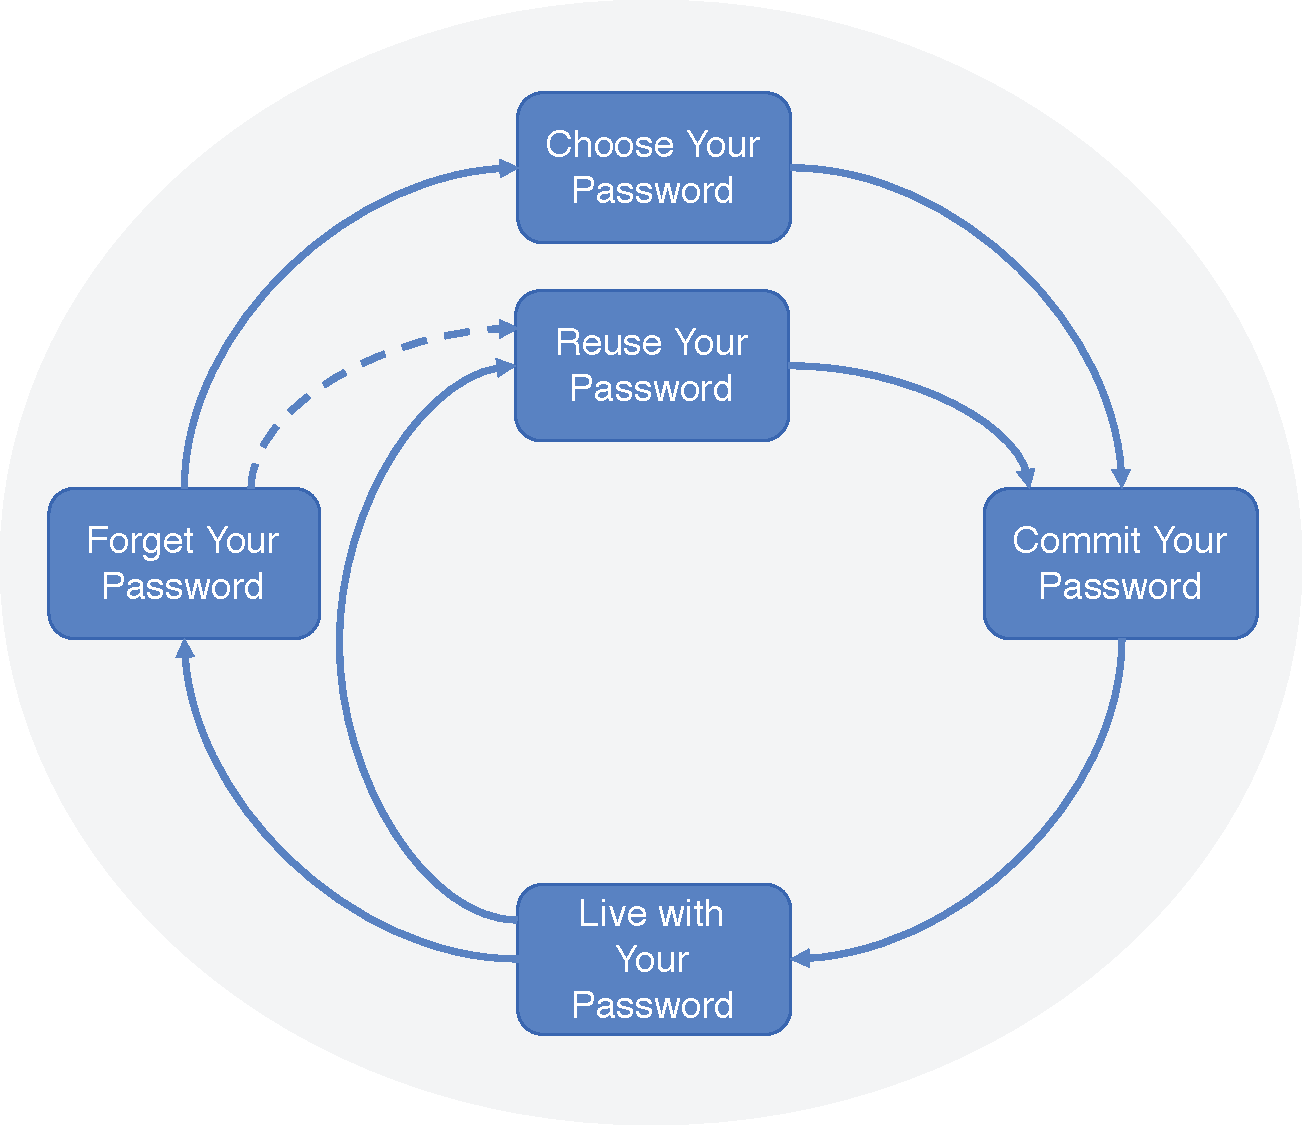
\includegraphics[width=0.65\linewidth]{rw/pw-life-cycle-new}
	\caption{\label{fig:rw:pw_life_cycle} Stobert and Biddle's ``Password Life Cycle'' \cite{Stobert2014PasswordLifeCycle} models typical stages of password behavior.}
\end{figure}

%TODO optional \todo{add a table that has all problems on one side and the possible user coping strategies on the other side.}

	\subsection{Weak Passwords}
	% things to answer in this section:
	% what's so difficult about selecting a strong password?
		% users do not see their passwords as predictable
		% users are too lazy. 
		% misconceptions about strength
	% what do users do if they want to select a strong password?
	% why don't they always do it?
	% when do they select stronger passwords?
	Why do users select weak passwords? 
	First of all, selecting a strong password is hard for most people. % I feel this lacks a reference ?
	Picking up the definition of a strong password (``something that is easy to remember, but difficult to guess'' \cite{Bishop1995ProactivePasswordChecking}), users do not struggle with the first part of the sentence, but the latter. Users do not intuitively know what makes a password \textit{difficult to guess} \cite{Jakobsson2013BenefitsUnderstandingPWs}, and not even security researchers reach ultimate consensus on that matter.  
	
	% users want MEMORABLE passwords.
	Let us look at the first part: something that is easy to remember. Numerous studies have looked at what people do to make their passwords easy to remember. For instance, personal information is easy to remember (``\texttt{TobiasSeitz}''), as is that of close ones (``\texttt{LenaSeitz}'') and pets (``\texttt{Fonsi\&Alois}'') \cite{Brown2004GeneratingPWs,Li2017PersonalInformation}. Veras \etal found that dates are very commonly found in passwords \cite{Veras2012VisualizingSemanticsPasswords}. Looking at the top 25 most-used passwords\footnote{SplashData publishes such a list each year, for 2017: \url{http://fortune.com/2017/12/19/the-25-most-used-hackable-passwords-2017-star-wars-freedom/} \la{12.01.2018}}, a list published after each public data leak, we can easily spot more patterns. One group consists of ``keyboard patterns'' (qwerty, qazwsx) and ``number sequences'' (12345, 123456, 1234567489, 1234567, 123123). The remainder fall into the ``likings'' (football, monkey, iloveyou, starwars, dragon) and ``password thematic'' (Password, letmein, admin, welcome, login, passw0rd, master, hello, trustno1) categories. All of these passwords are particularly easy to remember, which was quantified by Chiasson \etal \cite{Chiasson2009InterferencesGraphical}, but extremely predictable. However, they are often still allowed at many websites \cite{Seitz2017PoliciesReuse}. Interestingly, such password lists differ marginally across countries \cite{Violettas2014PasswordsAvoidGreece,Wang2015ChinesePWs}. Consequently, users' \textbf{desire to create memorable passwords} naturally leads to more obvious selections. 

%	pass\textit{word} implies it has to be a word. Other names for the concept, but basically the same meaning: security code, passcode, secret, credentials, access token

\begin{figure}[htbp]
	\centering
	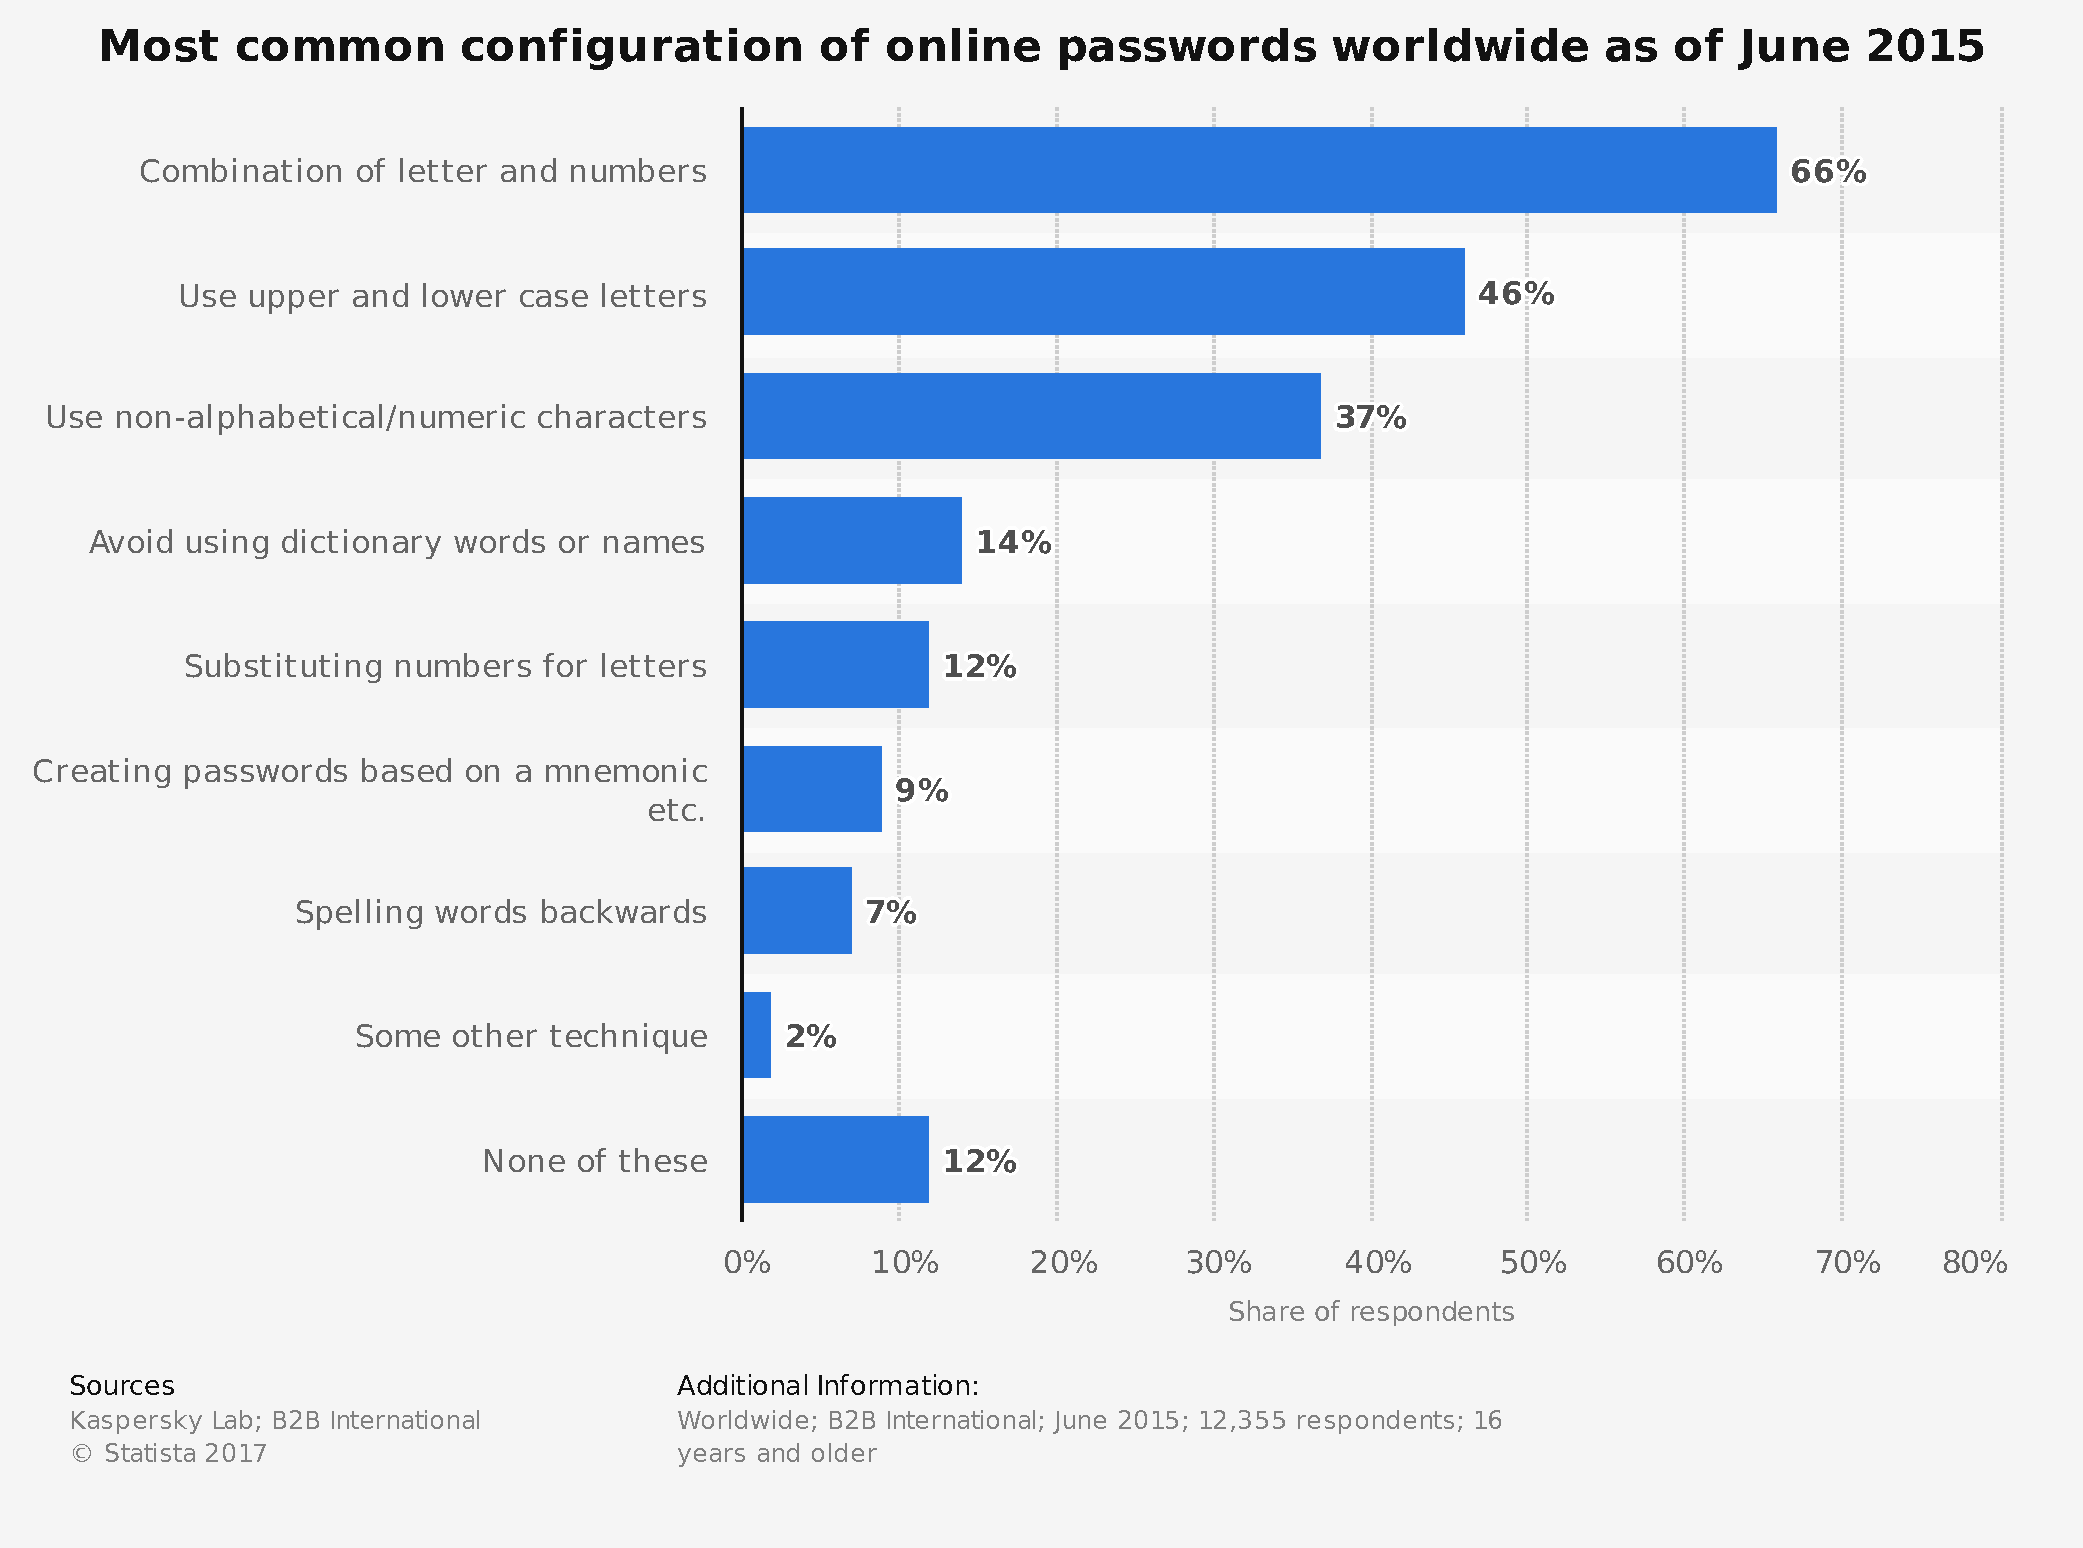
\includegraphics[width=0.6\linewidth]{../statista/statistic_id463406_typical-configuration-of-internet-passwords-2015}
	\caption{\todo{replace with own figure built from Kaspersky Lab report data} Survey results - how do people select their passwords (self report)}
\end{figure}
	
	% wrong mental model of strong passwords
	Another reason for the prevalence of weak passwords lies in incorrect \textit{mental models}. Mental models are descriptions of how humans make sense of functions and system states \cite{Volkamer2013MentalModels}. 
	%TODO better link to following text.
	Some users who aim to create stronger passwords still fail because their strategies to accomplish the task are predictable. Gaw \etal found that mangling is predictable \cite{Gaw2005ReuseRecycle}. Ur \etal pointed out that users understand a great deal of password security, but their modification behavior of existing passwords is sub-par \cite{Ur2015PWCreationLab}. Moreover, they provide evidence that users succeed to identify strong passwords, but only certain characteristics are misleading \cite{Ur2016PerceptionsPassword}. For instance, including digits yielded significantly higher subjective strength ratings, but does not always effectively improve strength. What is more is that participants in their study showed a skewed understanding of password attacks. (\todo{add example}) Therefore, their focus to fend off a dictionary attack might be futile if they do not know that attackers attempt to crack the password billions of times. Ur \etal conclude that feedback should thus inform users about attack scenarios which helps them assess the risk more realistically. Although it is sometimes argued that passphrases, i.e. a combination of multiple dictionary words, are often as secure as passwords from a richer character set \cite{Shay2012CorrectHorseBatteryStaple}, users fail to create strong passphrases, too. Bonneau studied the linguistic properties of passphrases at Amazon and noted that an attacker could easily model user behavior to effectively crack passphrases \cite{Bonneau2012LinguisticProperties}. So, in other words, the mental model ``passphrase = secure'' is also wrong and problematic. Finally, mental models also play a role for risk assessment in organizations. In many cases, employees underestimate the security threat that companies face day to day, which leads to insecure password practices \cite{Adams1999UsersEnemy, Weirich2001PrettyGoodPersuasion}. To summarize this point, users fail to create strong passwords, because in many cases \textbf{erroneous mental models} stand in the way.
	
	% laziness / rational rejection 
	What the media often call ``laziness'' and ``stupidity'' \cite{Volkamer2013MentalModels}, may in fact be the rational rejection of password security. Riley pointed out that users are well aware of ``better'' behavior, but they often ignore it by choice \cite{Riley2006WhatUsersKnowWhatTheyDo}. Florêncio \etal argue that this behavior is absolutely rational, because some accounts do not require strong protection and it would be impossible for users to follow all security advice given by experts \cite{Florencio2014PasswordPortfoliosFiniteUser}. A case example of an account that may be valuable for some, but not for others is LinkedIn. The social-media platform which is focused on business connections suffered a severe data breach in 2012, but only became aware of a much larger leakage in 2016. Many hashed passwords had leaked and thus the affected users were prompted to reset their passwords. Huh \etal investigated the reasons (not) to reset the password and in many instances, people said that they do not use the service very often, did not want to, or were not really concerned about the risks \cite{Huh2017TooBusy}. Ur \etal's results also indicate that users do know in theory what makes a strong password \cite{Ur2016PerceptionsPassword}. A survey commissioned by LastPass reported that one group of users often do not care about their accounts if they are not meaningful to them \cite{LastPass2016PersonalitiesGetUsHacked}, while the other group is overly careful, but there does not appear to be a ``just fine'' area of behavior. The first group may believe that stronger passwords do not accomplish protection anyhow \cite{Florencio2007DoStrongWebPasswords}. Herley and Pieters argue that it is also difficult to objectively falsify claims about security precautions, which would help to debunk unjustified security advice \cite{Herley2015Counterfactuals}. So, in essence, users choose weak passwords because they think \textbf{the account is unimportant} and therefore it is fine to ignore security advice.  
%	- people don't take password policies at organizations seriously.  \cite{Weirich2005PersuasivePasswordSecurity}

	% other factors
	Lastly, the literature lists a few other reasons that lead to weak passwords. Groß \etal looked at the association between cognitive depletion and selection behavior \cite{Gross2016EffectCognitiveEffort}. They reach the conclusion that if cognitively challenging tasks precede password selection, the resulting passwords tend to get weaker. Von Zezschwitz \etal point out that a user's first passwords are created probably in teenage years when security precautions might be much less evident to people \cite{VonZezschwitz2013SurvivalShortest}. For important accounts, these early passwords are modified, but still persist for many years after they were first committed to. 
	% Input modality - mobile devices
	Mobile phones are another factor that steadily gains more importance. Under lab conditions, Yang \etal found that participants included more lowercase letters in passwords, if they created them on a smartphone \cite{Yang2014EntryAffectsPasswordSecurity}. Von Zezschwitz \etal corroborate the findings and argue that passwords created on smartphones are much less diverse than their desktop-counterparts, because they are shorter and contain mostly lowercase letters \cite{VonZezschwitz2014HoneyIShrunkTheKeys}. Two years later, Melicher \etal studied the interoperability of passwords on different platforms \cite{Melicher2016UsabilityMobileTextPasswords}. Interestingly, the passwords created on mobiles were only marginally weaker than those created on a desktop, but had more potential to lead to user frustration, especially if requirements were too bothersome. The individual keyboard on a mobile influences frustration levels, too \cite{Haque2014PsychometricsStrongPassword}. 
	% Since biometric authentication prevails as unlock mechanism, the PINS and passwords users create as unlock protection tend to get weaker \cite{Cherapau2015ImpactOfTouchID}. 
	In summary, contextual factors like cognitive depletion and the device used during password creation have a notable impact on password strength. 
	%TODO consider: new character set: emojis. set the stage for the emoji passwords later. 
	
	% THEMES
	We thus identify four main themes from related work that cause weak passwords: 1) Weak passwords are more memorable. 2) Hard-to-change mental models prevent the creation of stronger passwords. 3) In many situations, users rationally reject the effort to create a strong password. 4) Contextual factors notably influence selection strategies. In the following, we dissect another coping strategy, which is potentially even riskier than selecting weak passwords: password reuse.

	\subsection{Password Reuse}
	% TOO MANY ACCOUNTS! Cannot remember them!
	The primary reason for password reuse is the mere fact that users create new accounts on a regular basis, and it is logical to make sure to be able to log in later by choosing a secret they already know. ``Password overload'' essentially frames the problem \cite{Yang2016MnemonicSentenceBased}. ``Memory interference'' postulates reuse as a coping strategy \cite{Chiasson2009InterferencesGraphical}. In 2007, Florêncio and Herley conducted a large-scale study that empirically showed the challenges and coping strategies regarding this overload \cite{Florencio2007LargeScaleStudyPasswordHabits}: Users of the Windows Live Toolbar had 6.5 distinct passwords, each of which was used for 3.9 different websites. During the data collection period, users logged into 25 accounts on a regular basis, and typed around 8 passwords per day. Although keeping track of the multitude of username-password combinations is a tough challenge, most users still rely on their memory instead of other tools \cite{Olmstead2017AmerciansCybersecurity}. Users realize the challenge is hard, but Woods \etal argue that users underestimate their capabilities when it comes to memorizing passwords \cite{Woods2018TooManyPasswords}. Consequently, many people do not try to create a richer portfolio of passwords than the numbers from the 2007 study showed. More recent numbers show that between 39\% \cite{Olmstead2017AmerciansCybersecurity} and 76\% \cite{CSID2012PasswordHabits} of users rely on reuse as coping strategy. Since social desirability bias could lead to dishonest survey responses, the ``dark figure'' might even be higher, because, as Inglesant and Sasse put it, ``\textit{Users see `good' passwords (that are memorable and conform to the policy) as a `resource', which they continue to use for new applications even if the original use is no longer allowed.}'' (\cite{Inglesant2010TrueCostOfUnusablePolicies}). What is more is that the user-name is part of the authentication process, and users pick different aliases, pseudonyms, emails for different accounts \cite{Hayashi2011DiaryStudyPWs}.
	
	All this is consequential for the overall online security of an individual. The more a user relies on reuse passwords, the more severe phishing attacks and data breaches become. The metaphorical ``Domino Effect'' describes the situation after a breach: When an attacker obtains a password form one user's account, all the other accounts might fall with it \cite{Ives2004DominoEffectReuse}. It's enough to know even only one low-value password to crack a large part of high-value passwords via predictable mangling rules \cite{Das2014TangledWeb, Haque2014Hierarchy}. Still, password reuse is difficult to mitigate, so Ives argues to look into understanding the specific approaches better \cite{Ives2004DominoEffectReuse}.
	
	% organize reused passwords:
	% categories
	One such approach is to categorize passwords by different criteria. Here, we can borrow the ``Mental Accounting'' theory from Behavioral Economics to describe users' risk assessments. \cite{Stockinger2015TowardsBE,Thaler2004}. Users put their passwords into mental accounts that help them recall them later. 
	% frequency
	Wash \etal argues that frequently entered credentials are reused more likely than seldom used ones \cite{Wash2016UnderstandingPasswordChoices}. However, interviewees in Stobert and Biddle's study reported the opposite behavior \cite{Stobert2014PasswordLifeCycle}. 
	% strength
	Florêncio and Herley noticed that strong passwords (in terms of entropy) are less frequently reused than weak passwords \cite{Florencio2007LargeScaleStudyPasswordHabits}. Here again, Wash \etal observed the opposite: participants in their study prioritized stronger passwords as reuse candidates \cite{Wash2016UnderstandingPasswordChoices}. If the latter is true, than this is another indicator for problematic mental models regarding risk assessment: users try to follow security advice and prefer strength over uniquenessm which is typically also advised. Nonetheless, strategies (or at least results) appear to fluctuate throughout the years. 
	% value
	Many users cluster their secrets regarding the usage purpose \cite{Haque2014Hierarchy}, e.g. banking, social media, communication, shopping, etc. \cite{Notoatmodjo2007ExploringWeakestLink,Stobert2014PWMThatDoesntRemember}. Bailey \etal, however, argue that users do not really respect the usage purpose, but the value, importance, and meaningfulness of the account \cite{Bailey2014StatisticsReuse}. In that sense, users do not appear to care if the password ought to protect financial information if the website does not mean much to them. Radke \etal found users in their diary study tended to create unique passwords for important accounts, and reuse passwords for less important ones \cite{Radke2013WhoDecides}. Still, probably all users have a ``go-to password'' that is tried first for an account whose value is uncertain in the beginning \cite{Stobert2014PasswordLifeCycle}. 
	% reuse with modifications
	If password requirements disallow the preferred choice, the go-to password might not work anymore. Typically, users either pick another password from their portfolio in that situation, or they mangle their first choice until all requirements are met. As we show in Chapter \ref{chap:policies-reuse}, neither strategy is necessary if the go-to-password shows certain features. But in case the policy mandates a change, Gaw and Felten have laid out that user-chosen mangling strategies are predictable, too \cite{Gaw2006PasswordManagement}. Besides, policies might not be the only reason for password modifications. Over time, users sometimes are exposed to new security advice or other realizations that their previous password strategy is generally considered weak \cite{VonZezschwitz2013SurvivalShortest}. Taking the current (already memorized) credentials, and applying the recommendations to them is an obvious choice. 
		
	% expert behavior
	Florêncio \etal describe reuse, categorization, memorable passwords, and mangling as ``finite effort'' \cite{Florencio2014PasswordPortfoliosFiniteUser}. They meticulously lay out that password these strategies are not only common, but inevitable and necessary. Even experts in cybersecurity show similar patterns \cite{Loutfi2015PasswordsOtherSideOfTheFence,Stobert2015ExpertPassword}. The major difference between mainstream users and experts is that the latter are more articulate and considerate about their coping strategies. 

%	A new scale and insights into password support. Password hierarchy \cite{Haque2015PhdProposal}
	
	% summary
	In conclusion, we can hang on to the idea that password reuse is a necessary coping strategy. Zhang-Kennedy \etal motivate that it is not even ``bad'' or ``risky'' per se \cite{ZhangKennedy2016RevisitingPasswordRules}. The challenge is to do it ``right''. However, motivating users to alter this particular aspect is comparable to motivating a smoker to quit their guilty pleasure: Abandoning reuse does not show a visible immediate pay-off (nor does quitting smoking). In many cases, it does not cause harm, even though 16\% of US-Americans have experiences someone else taking over their accounts \cite{Olmstead2017AmerciansCybersecurity} (a similar percentage of active smokers develop lung cancer\footurl{https://www.verywell.com/what-percentage-of-smokers-get-lung-cancer-2248868}{13.01.2018}). 
	
	
	\subsection{External Storage}\label{sec:rw:external-storage}
	%Write down passwords.	
	To avoid memory interference, many users resort to writing down their passwords. In its simplest form, a sheet of paper that holds user name and password suffices. Roughly half the users reportedly do this \cite{Olmstead2017AmerciansCybersecurity}. Many users also use a dedicated note-book that keeps their passwords in one place \cite{Kothari2017PasswordLogbooks}. Interestingly, some manufacturers offer ``password-logbooks'' to help users organize their credentials. Kothari \etal collected customer reviews about the ten most reviewed logbooks and analyzed their content to derive a mental model of password security \cite{Kothari2017PasswordLogbooks}. They were surprised how many people apparently use one of those logbooks and what their motivations are. For instance, customers often loved the inconspicuousness of the books and gave them away as presents. Age-related memorability challenges were also a central theme. Many people acknowledged the security risks but were unsure if a piece of software would be more secure than the book. Password logbooks can become a single point-of-failure. Digital files on the computer are often almost as accessible to local attackers (friends / spouses). In the workplace, writing passwords down on sticky notes \cite{Conklin2004PWAuthenticationSystemPerspective} leaves the credentials wide open to anyone passing by and enforcing different behavior is difficult. Nevertheless, Herley and Van Oorschot generally advocate writing down as coping strategy, as long as the notes are stored in a fairly secure location \cite{Herley2012PersistenceOfPasswords}.  

	% PASSWORD MANAGERS
	Using a \gls{PWM} is a more sophisticated way of ``externalizing'' passwords. In essence, a password manager is a digital representation of the ``logbooks'' described above, but comes with many helpful extra features, like easy access, encryption with a master password etc. A plethora of services and tools exist in different flavors (e.g. built into browsers, third party programs, browser extensions, free vs. premium, cloud-based vs. local). Notable representatives include LastPass (freemium/subscription), 1Password (premium/subscription), KeePassX (free, one-off payment for apps), and Dashlane (freemium/subscription). Arias-Cabarcos \etal evaluated popular PWMs and suggest that Dashlane provides the the most feasible usability/security trade-off \cite{AriasCabarcos2016ComparingPWM}. However, surveys have often revealed the low adoption rate of password managers \cite{Olmstead2017AmerciansCybersecurity}, mostly because users feel secure enough with their current management habits, or due to financial hurdles and distrust \cite{CSID2012PasswordHabits,Fagan2017UsersConsiderationsPWMs}. 
	
	% PWM benefits and drawbacks
	Lyastani \etal recently investigated the impact of using a PWM on password strength and reuse \cite{Lyastani2017ImpactPWMPasswordStrength}. Those \glspl{PWM} which included a generator had a positive effect on overall password strength and diversity in the large sample studied in-situ. But existing user strategies thwarted a boost in security, e.g. if a built-in \gls{PWM} is solely used to store reused passwords. Users often benefit from automatically filled login-forms and do not have to type their passwords anymore, which is a huge usability plus. Autofill moreover mitigates most phishing attacks, because the \gls{PWM} verifies the domain. As with analog notepads, PWMs are a single point of failure, in case the master password is weak. This is one of the few instances in which a strong password is recommended without restrictions. Password managers constitute a honey pot for attackers, who exploit security vulnerabilities of the software to gain access to user passwords \cite{Bonneau2012ReplacePasswords}. The situation is aggravated if passwords are synced to the manufacturer's cloud storage, although this is recommended by Yee to enable seamless availability \cite{Yee2006Passpet}. To summarize, password managers are a feasible solution for many users, but adoption rates are still fairly low. 

	\subsection{Fallback Methods}
	Coping with a forgotten password shows more particularities of user behavior. If offered by \glspl{SP}, the easiest way to handle the situation is to obtain a password reset link via email and create a new password. In the past, password resets had been responsible for a large portion of helpdesk calls \cite{Sasse2001WeakestLink}, but self-service procedures have successfully mitigated the issue. Users tend to reuse passwords or mangle an old password when they forget and reset their credentials \cite{Stobert2014PasswordLifeCycle}. In some cases, however, password reset links are replaced by personal knowledge questions \cite{Bonneau2015SecretsLies}. These often present a great risk to user accounts because of the statistical probability involved (e.g. ``what was the make of your first car'' has a predictable distribution), or the information is findable on social networks (e.g. ``what is your city of birth''). Consequently, a strong primary password can be dominated by a weak fallback question and voids user efforts to secure their account. Perhaps the only strategy to maximize security within this scheme is to provide bogus answers to secret questions to fend-off statistical attacks \footurl{https://lifehacker.com/use-fake-answers-to-online-security-questions-1821628011}{14.01.2018}. 

	\subsection{Account Sharing}
	Users often share their accounts, e.g. with close-ones, relatives, or co-workers \cite{Kaye2011PasswordSharing, Shay2010EncounteringPasswordRequirements}. Security advice generally discourages sharing passwords because it increases the likelihood of leaked credentials. However, Singh \etal point out that this behavior is absolutely intentional, and does not originate from lack of understanding the risks involved \cite{Singh2007PasswordSharing}. Password managers also integrate sharing features to give others quick and easy access to a set of passwords \cite{Li2014EmperorsNewPWM}. Account sharing plays a role in the overall security strategy, but personal passwords are usually less influenced by sharing considerations. 

	\subsection{Summary}
	We can identify themes in coping strategies at each stage of the Password Life Cycle \cite{Stobert2014PasswordLifeCycle}. Coping is a natural reaction to ``impossible demands'' arising from Password overload \cite{Sasse2005UsableSecurityPosition}. All strategies can be justified from an economic point of view \cite{Florencio2014PasswordPortfoliosFiniteUser}, although each of them generates security risks of varying severity. Password reuse is arguably the most severe problem, followed by selecting too obvious and weak passwords. It is critical to be consistent with one's own reuse strategy and pick strong passwords in a select number of cases, e.g. master passwords for \glspl{PWM} or central hubs like email accounts. In the following, we discuss how research has tried to influence risky behavior and support users in safe behaviors. 

%%%%%%%%%%%%%%%%%%%%%%%%%
%%%%%
%%%%% COUNTERMEASURES
%%%%%
%%%%%%%%%%%%%%%%%%%%%%%%%
\section{Guiding and Aiding Users}\label{sec:rw:user-support-interventions}
Since secure behavior does not come natural to users, there have been many attempts to make it more accessible to them and relieve the tensions between usability and security at the same time. Although systems can be changed in many ways, it is difficult to change the user. If the user needs to be kept in the loop, e.g. because constraints dictate so, we need to support them well and make careful decisions about how to support them \cite{Cranor2008FrameworkReasoning}. In the following, we highlight approaches not only to make systems more usable, but also to influence user behavior regarding passwords. 
%Usable security shouldn't only be done for end users but also for the people who implement security systems \cite{Acar2016NotYourDeveloper}
	\subsection{Password Composition Policies}\label{sec:rw:policies}
	%Lingo: Adhere to a policy
	% history, where did the idea originate?
	Combating weak passwords has received the most attention from research and practice. The idea of enforcing certain password requriments dates back to the 1970s, i.e. the early days of cybersecurity. Morris and Thompson acknowledged password authentication is inherently flawed in terms of usability. They suggested to make users either choose longer passwords, or systematically assign passwords to them to \cite{Morris1979PasswordSecurity}.
	At the time, guessing attacks were not as powerful as they are today and it was obvious to shift responsibility to users \cite{Feldmeier1990UnixPasswordSecurity}. When the Electronic Authentication guideline was published by \gls{NIST}, password composition policies became the de-facto standard in attempting to make users select stronger passwords. The NIST guideline suggested passwords be at least eight characters long, include at least one upper case letter, one lower case letter, one digit, and one special symbol \cite{Burr2004NISTEntropy}. Moreover, passwords may not be taken from a dictionary with common words and not be permutations of the username. By looking at entropy estimates, it was argued that the resulting passwords would achieve at least 30 bits of entropy. Interestingly, this was not the only specification for policies. The guideline specifically says that passwords could also be graded with some other metric and be rejected based on their estimated entropy. At the time, there was not much evidence that user-selected passwords created under the NIST-policy were in fact strong, which set of a number of research studies, and made password composition policies one of the most studied topics in password security. 

	Proctor \etal found in 2002 that certain ``proactive password restrictions'' lead to stronger passwords \cite{Proctor2002ImprovingAuthenticationProactivePasswordRestrictions}. In two laboratory experiments, they had participants create a new password for a university account. The policies differed in the required minimum length (five and eight) and additional requirements like upper-/lowercase letters and digits. In the first experiment, where passwords only had to be five characters long, introducing the additional requirements had a greater effect on strength than in the eight-character-minimum condition. Increasing the minimum length by three characters already had a stronger effect. Interestingly, they concluded ``Perhaps the most important message of this study is that restrictions on user-generated passwords may not accomplish their intended goals.'' Proctor \etal's early hypothesis that policies are more or less ineffective is particularly surprising because in the fifteen years that followed, many research papers were written about such restrictions and many of them ultimately came to similar conclusions. In the following some of the most influential works are summarized.
	
	%now we need to report on a couple of papers that come to the conclusion that policies are somewhat ineffective.	
	Inglesant and Sasse report on a diary study of password policies in corporate contexts \cite{Inglesant2010TrueCostOfUnusablePolicies}. They reached the disillusioning conclusion that password policies reduce employees' productivity. Once they found a password that fulfilled the policy, participants used it as a resource to turn to when creating more accounts. Similarly, Komanduri found that users barely go beyond the minimum requirements of policies \cite{Komanduri2011OfPasswordsAndPeople}, but some policies yield better results than others. %The idea of a holistic password policy is put forward 
	Weir \etal categorize policies into ``explicit'' and ``implicit'' policies \cite{Weir2010MetricsPolicies}, where explicit policies have predefined rules about the password structure like the NIST policies which is explicitly based on \gls{LUDS} \cite{Wheeler2016zxcvbn}. On the other hand, implicit policies focus on strength estimation and are somewhat more volatile and intransparent to the users. For instance, if the policy uses a blacklist of words, that are disallowed, the list is usually not displayed to users up front. The blacklist only becomes visible after the first attempt is made. Moreover, they used subsets of the RockYou data set that fulfilled the NIST policy. Here, Weir \etal provided early pointers that many of those passwords can be easily cracked, too. 
	
	Thus, the logical next step was to find replacements for the NIST policy with better usability and security. First attempts to find it were of theoretical nature. Blocki \etal modeled an ``optimal'' policy as algorithmically solvable challenge \cite{Blocki2013OptimizingPasswordPolicies}, which was proposed by Shay \cite{Shay2009PolicySimulation}. However, while theoretically sound, empirical evidence was necessary to quantify the effects on user behavior. 
	%There are also ``external'' policies where the user's password is automatically changed by the system to add some randomness

	% GUESS NUMBER GRAPH
	\begin{figure}[!htbp]
		\centering
		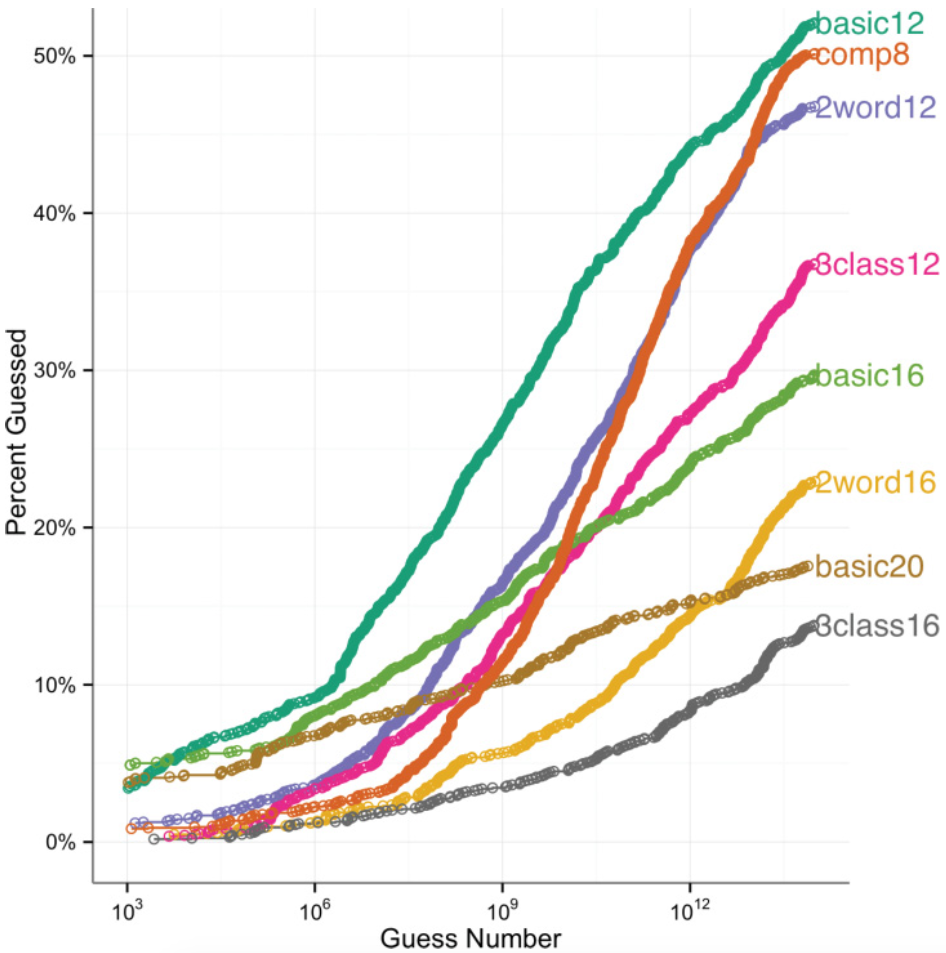
\includegraphics[width=0.6\linewidth]{rw/guess-number-graph}
		\caption{\label{fig:rw:guess-number-graph} Guess number graph for passwords created under different password composition policies. A higher percentage of cracked passwords (larger y-values) indicates that passwords were weaker. In this case, passwords adhering to a basic12 policy were the weakest, while 3class16 produced the strongest passwords.}
	\end{figure}
	During the last few years, Shay \etal have established a taxonomy for policies \cite{Komanduri2011OfPasswordsAndPeople, Shay2014CanLongPasswordsBeSecureAndUsable,Shay2016DesigningPasswordPolicies}: Basic policies that only mandate a certain length (e.g. basic12), character-class centric policies that require between 2 and 4 different character classes and a given length (e.g. 3class12), policies requiring phrase-like syntax and a given length (e.g. 2word16), and complex policies that have more than 4 specific requirements (comp8). Table \ref{tab:rw:policy-descriptions} illustrates the specific differences as found in the taxonomy. In multiple studies they compared the guessability of passwords under different policies. They found that a 3class16 policy produced the least guessable passwords, while basic12 yielded the highest cracking success rates. For a limited attacker, who can make up to $10^6$ guesses, basic16 and basic20 performed poorly, but they fared well at the cut-off threshold of $10^{14}$. The NIST-policy (comp8) performed well up to $10^6$ guesses, but almost as many passwords had been cracked after $10^{14}$ guesses as for the basic12 policy. This refutes the postulation that character diversity automatically leads to stronger passwords when users select them. Shay \etal point out that 28\% in the comp8 condition only fulfilled the criteria by adding an exclamation mark ``!'' at the end, which is corroborated by Ur \etal \cite{Ur2015PWCreationLab}. So, as hypothesized, policies significantly influence the strength of user-generated passwords. In terms of usability, there are signficant differences, too. Shay \etal examined typical usability metrics, as well as user ratings. basic12 passwords were the easiest to create, fastest to type and easiest to remember. Interestingly, the 3class12 policy was comparable in all dimensions. All in all, basic16, 3class12, and 2word16 seem like the ``winners'' in terms of security and usability, but 2word16 passwords have high beta guess rates \cite{Shay2014CanLongPasswordsBeSecureAndUsable}. To combat this, Shay \etal suggest blacklisting specific sub-strings \cite{Shay2016DesigningPasswordPolicies}.
		
	% Table tab:rw:policy-descriptions
	% POLICY descriptions
	% Table generated by Excel2LaTeX from sheet 'policy taxonomy'
\begin{table}[htbp]
  \centering
  \caption{\label{tab:rw:policy-descriptions} Example policies from CMU taxonomy. }
    \begin{tabular}{lp{7.5cm}p{4cm}}
    \textbf{Policy} & \textbf{The password needs to ...} & \textbf{Example passwords} \\ \hline \hline
    basic8 (1class8) & be at least 8 characters long & password \linebreak monkey123 \linebreak qwerasdf \\ \hline
    3class12 & be at least 12 characters long and include three different character classes (upper, lower, digits, symbol) & Password1234 \linebreak 2MonkeysBite \linebreak NfJidl2kdils \\ \hline
    2word16 & be at least 16 characters long and include at least two letter sequences that are separated by a non-letter sequence. & password.unlocks \linebreak 1-Monkey-Bites \linebreak qwer.asdf.zxcvb.1234 \\ \hline
        comp8 & bet at least 8 characters long, include at least one character from each character class, and not include a dictionary word & P@ssw0rd \linebreak !M0nkey1 \linebreak LGtjj\{Rd;w1u/ \\ \hline \hline
    \end{tabular}%
\end{table}%


	% Policies influence security and usability, meters are often ineffective because only stringent meters seem to work \cite{Ur2012HelpingUsersCreateBetterPasswords}
	
	%The authors present how they would design an experiment about persuasive messaging, but didn't really carry it out (and the method doesn't seem suitable) \cite{Zakaria2013DesigningEffectiveSecurityMessages}

	% password expiration policy
	In the industry and public institutions, password expiration policies are commonplace  \cite{Inglesant2010TrueCostOfUnusablePolicies,Chiasson2015QuantifyingExpiration}. Forcing users to reset their users in predefined intervals was argued to mitigate threats arising from data breaches. If password leaks go unnoticed, at least they expire at regular points. For users, an expiration policy drastically increases password overload and memory interference, for which the typical coping strategies (see Section \ref{sec:rw:user-behavior}) prevail: an expired ``password1'' quickly is reset to ``password2'' and so forth \cite{Zhang2010PasswordExpiration}. Thus, it has been argued that expiration is ineffective and causes users too much effort without graspable security benefits. Chiasson \etal set out to quantify the benefits of expiration but their mathematical model strongly indicated that the benefits are ``marginal at best'' \cite{Chiasson2015QuantifyingExpiration}. If expiration is not enforced, security experts often advise users to change their password often. Zhang-Kennedy \etal reframe this rule to ``change your password well'' \cite{ZhangKennedy2016RevisitingPasswordRules}, i.e. users ought to change it once they suspect (or find out) a service had been compromised.
	
	% more nudging - focused: Penalizing users by making them wait can be a strong nudge to comply and create a stronger password \cite{Malkin2013Waiting}
	
	% state of the world: policies in the wild 
	Looking at real-world policies, Wang \etal also find inconsistencies, i.e. not all web sites require the same password characteristics	\cite{Wang2015EmperorsPolicies}. Users can get confused if multiple sites mandate different features for ``security reasons'', because they might wonder who is right. Florêncio and Herley compared policies of high-traffic websites and public institutions, mostly universities \cite{Florencio2010WhereDoPoliciesComeFrom}. Surprisingly, the most influential companies enforce some of the loosest policies. The researchers argue that decisions in these companies are not only influenced by security officers (who evangelize password strength and expiration) but also by user experience experts (who point out the usability issues). In public institutions, security advisors outnumber human-factors experts, which is why policies represent an ``overshoot'' of security there, imposing considerable nuisance at marginal security benefits. 
	
	% summary:
	To summarize, policies have power to influence password behavior. However, this influence arises from coercion and thus risks reduced usability. Users often cope by picking the easiest possible password that still fulfills the rules. This is why Florêncio \etal argue that we should not try to fix the user, but to fix the system (in this case policies) first \cite{Florencio2014AdministratorsGuide}. Especially, \glspl{SP} should be careful not to impose strict requirements and nonsensical policies\footnote{An amusing collection of nonsensical policies is collected on \url{https://twitter.com/PWTooStrong} \la{14.01.2018}}. However, if \glspl{SP} feel the need to move to a stricter policy (and expire passwords at the time of policy change), Shay \etal at least provide evidence that users feel better protected afterwards, even though their password changes are well predictable \cite{Shay2010EncounteringPasswordRequirements}. Finally, \gls{NIST} recently recognized that errors were made in the Electronic Authentication guideline and released an updated version \ar. William Burr, who was the lead author of the original policy recommendation, was recently quoted to regret his contribution. He told the Wall Street Journal ``\textit{It just drives people bananas and they don’t pick good passwords no matter what you do}''\footurl{http://fortune.com/2017/08/07/password-recommendation-special-characters/}{14.01.2018}. Shay \etal's results, however, somewhat relieve Burr from his remorse, because some policies help people pick ``good passwords''.
	
	%TODO cite Mayer \etal 2017 (similar to our password audit)
	%TODO real time feedback in policy fulfillment could actually go here instead of the persuasion section
	
	% USER EDUCATION / ADVICE / GUIDES 
	\subsection{User Education and Guidelines}\label{sec:rw:advice_guidance}
	Policies can be considered a means to ``enforce recommendations''. However, giving advice to users to educate them about password security is a softer approach. A Google search for ``password recommendations'' yields $\approx$ 113,000,000 results, some very brief\footurl{https://www.ibm.com/support/knowledgecenter/SS42VS_7.2.7/com.ibm.qradar.doc/c_qradar_niap_password_recommendations.html}{15.01.2018}, others very elaborate and authoritative\footurl{https://www.ncsc.gov.uk/guidance/helping-end-users-manage-their-passwords}{22.12.2017}. We summarized common advice and the characteristics of ``bad passwords'' in Section \ref{sec:rw:whats_a_bad_pw}. The original \gls{NIST} guideline also read more like a ``how to'' than a dictum for policies, although it was translated into policies after all. Sasse \etal expressed doubts about the effectiveness of user education, because it ``will only work if users are motivated'' \cite{Sasse2001WeakestLink}. We know by now that security is a secondary goal, and thus it is unlikely that people are motivated to educate themselves about it. Therefore, we have to focus on the restriction ``if users are motivated'' and present advice effectively in this opportune moment. Security can become the primary task, or on-par with the primary task. For instance, the moment users adopt a password manager and have to set-up their master password, they not only want to simplify password management, but also ensure that their central hub is safeguarded against attacks. Some web-accounts are of great value and users are potentially more open to receive support to secure those. 
	
	% positive examples, work that argues in favor of education
	% make education ``persuasive''  \cite{Zakaria2013DesigningEffectiveSecurityMessages}
	
	% issues with education
	We can identify four central problems with password advice. 
	% 1) there is no consensus
	1) There is no consensus about adequate password strength, because it always depends on the attack model. Thus, any guideline should differentiate between threat models and brief the users about them. However, this is rarely done in practice and most advice is opinionated \cite{Herley2015Counterfactuals}. Besides, password advice becomes outdated if new threat models prevail.
	% 2) understanding/knowledge does not translate into action
	2) Reading a guide does not necessarily translate into action. Herley says users are rational in rejecting advice if it entails too much effort \cite{Herley2009SoLongThanksExternalities}. Forget \etal empirically showed that advice can lead to insecure behavior, too \cite{Forget2007HelpingUsers}. 
	% 3) advice is forgotten and badly recalled later. Advice leads to wrong mental models
	%\paragraph{Password advice considered harmful}
	3) Users misread password advice. Ur \etal argue that users misconstrue a statement like ``adding digits, upper-case letters, lower-case letters and symbols add to the strength of the passwords'' to ``\textit{all} passwords with digits, upper and lower case letters, and symbols are strong'' \cite{Ur2016PerceptionsPassword}. Heterogeneous composition policies, and feedback can influence mental models, too.	Forget \etal argue that one needs to understand users' mental models of authentication first, before they can be effectively instructed \cite{Forget2007HelpingUsers}.
	% 4) all advice will translate into attacks that incorporate the same advice.
	4) Lastly, if password advice achieves to change user behavior on a larger scale, password guessing attacks will be modeled around the recommendations, too \cite{Herley2012PersistenceOfPasswords}. Thus, in the long run, advice needs to be revised because attacks become too efficient.
		
	%In privacy: people's mental models about privacy are vague and we can see it in their drawings/explanations that they're somewhat overly pessimistic and that education plays the major role \cite{Kang2015MentalModelsDrawing}
	
	To conclude, one needs to stay realistic about what can be achieved with password advice \cite{Florencio2016CommACM}. Zhang-Kennedy \etal provide this realistic view on advice \cite{ZhangKennedy2016RevisitingPasswordRules}. They revised the ``character diversity'' recommendation and suggest not using common passwords, predictable substitutions, or dictionary words. However, we still face the problem of communicating to users what ``common'' passwords and ``predictable substitutions'' are. Zhang-Kennedy \etal propose users should come up with original mnemonics, which is a special kind of advice discussed in the following. 	
		
	%%%%%
	%%%%%	Algorithms and Memorization Techniques
	%%%%%
	\subsection{Password Selection Algorithms \& Memorization Techniques}
	Many researchers have proposed techniques and algorithms to help users create memorable and strong passwords. Haskett put forward PassAlgorithms \cite{Haskett1984PassAlgorithms}, where the user remembered how to respond to a challenge rather than a static password. 
	\paragraph{Mnemonics and Training}
	Barton and Barton were likely the first to propose mangling strategies in this context \cite{Barton1984Mangling}. For instance, they suggested to use sentence-based mnemonics and mentally connect passwords to different cities. For Paris, a sentence like ``I love Paris in the Springtime'' would translate into ``IlPitS''. This work was seminal and some of its techniques persist in password recommendations today. Yan \etal empirically showed the benefits in terms of memorability and security of the resulting passwords \cite{Yan2004PasswordMemorabilitySecurity}. However, Forget \etal observed that telling participants to generate phrase-based passwords can be misinterpreted and more guidance is necessary to achieve benefits \cite{Forget2007HelpingUsers}. Maqbali \cite{Maqbali2016PasswordGenerators} and McEvoy \cite{Mcevoy2016ContextualizingMnemonicPhrase} recommend using contextual or site-specific cues on websites as mnemonics. 
	
	Memorization by repetitive training has also been suggested. Bonneau and Schechter put forward solution that is supposed to help users memorize ``56 bit secrets'' (for comparison, the original NIST guideline demanded 30 bit) \cite{Bonneau2014ReliableStorage56Bits}. Users first pick a self-selected password. They system then displays a random code (or words) for each user at login-time which needs to be typed correctly into a separate field. The code becomes part of the password and was displayed with increasing delays. But participants could skip the delay by entering the code from memory. After a median of 36 log-ins 96\% of participants had memorized a 56 bit secret. Despite the high success rates, it is questionable if this type of aide is in the users' interest, especially if it is deployed by more than one service. In a similar vein, Kroeze and Olivier proposed using gamification to make the training more enjoyable \cite{Kroeze2012GamifyingAuthentication}.
	
	%	Yet another memorization aid - work in progress \cite{Lyastani2016PWMangling} 
	In terms of security, mnemonic passwords are predictably based on common phrases from movies, literature, songs, etc., but stronger than intuitively selected passwords \cite{Kuo2006HumanSelectionMnemonic}. Yang \etal demonstrate that even mnemonic phrase-based passwords can be attacked easily \cite{Yang2016MnemonicSentenceBased}. Thus, like Zhang-Kennedy, they highlight the importance of original, personal phrases and show how users can be instructed effectively.
		
	%In a convenience sample, persuasive text passwords were sufficiently memorable \cite{Forget2008MemorabilityPersuasivePasswords}	
	
	\paragraph{Passphrases}\label{sec:rw:passphrases}
	Another technique proposed to create strong, memorable passwords is to create passphrases. Rather than taking single letters from a phrase, we understand them as a combination of words, e.g. the paragon ``\texttt{CorrectHorseBatteryStaple}''. Passphrases are usually longer than traditional pass\textit{words} and thus increase password strength. The PGP system uses passphrases to encrypt private keys on the clients. Keith \etal showed that, at the same time, passphrases are more memorable than more complex passwords, especially if they include punctuation symbols \cite{Keith2009PassphraseDesign}. However, participants in their study made significantly more errors, which is the biggest usability caveat of long passphrases. On devices where text-entry is cumbersome (e.g. on mobiles or smart TVs), refraining from masking entry can mitigate this problem \cite{Melicher2016UsabilityMobileTextPasswords}. Paradoxically, passphrases sometimes exceed character limits for passwords on certain websites \cite{Carnavalet2014AnalyzingPWStrengthMeters}. 
	
	Moreover, Bonneau showed that user-selected passphrases are predictable \cite{Bonneau2012LinguisticProperties}. To mitigate predictable word combinations, system-assigned passphrases have been evaluated. Shay \etal conclude that this boosts strength, but users dislike them \cite{Shay2012CorrectHorseBatteryStaple}. Similarly, policies focused on passphrases (e.g. 2word16) lead to passwords with high guess numbers, but users struggle to create them \cite{Shay2014CanLongPasswordsBeSecureAndUsable}. The Diceware approach is often mentioned as a means to randomize word selection \footurl{http://world.std.com/~reinhold/diceware.html}{16.01.2018}. The user rolls a dice firve times and notes down the resulting numbers. Afterwards, they look up the word with the corresponding number from the Diceware wordlist. The process should be repeated at least twice to create a passphrase. Unfortunately, the process requires some dedication, time, and a dice. Nonetheless, passphrases usually do not require a change to the provider's system, which makes them a viable, memorable and secure option, e.g. if they are mostly entered with a physical keyboard. 
	
	%Advantages: PW scheme doesn't have to be changed, people are generally familiar with the concept of passwords, better to enter on virtual keyboards, e.g. TVs (although we don't have any data for that, but that's okay because passwords play a minor role (but still exist there)).
	
	%%%%%%
	%%%%%% Password Managers and Generators
	%%%%%%
	\subsection{Password Managers and Generators}\label{sec:rw:pwm_generators}
	%TODO I'm not quite sure how to avoid redundancy here. 
	\todo{careful: this section must not get too redundant}
	Many of the problems around password security originate from the predictability of user choices and preferences. Therefore, systems that remove the decision-making process for a large part seem to remove weak passwords. Password generators can create (pseudo-)random strong passwords for the users and thus the element of human bias vanishes. There are different approaches to generate passwords for users under two paradigms: easily memorable passwords, or passwords requiring external storage (see Section \ref{sec:rw:external-storage}). 
	% password generator figures. TODO use subfigures.
	\begin{figure}
		\centering
		%TODO we could use Dashlane's screenshot here. 
		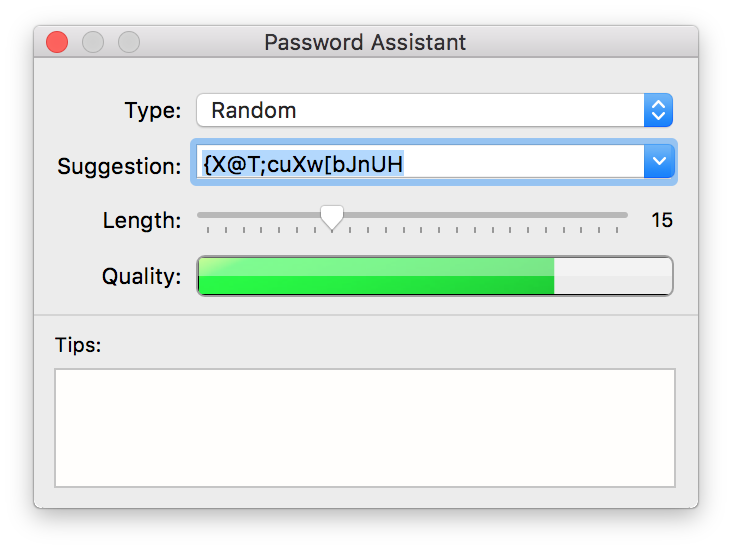
\includegraphics[width=0.49\linewidth]{rw/apple-pw-assistant-random}
		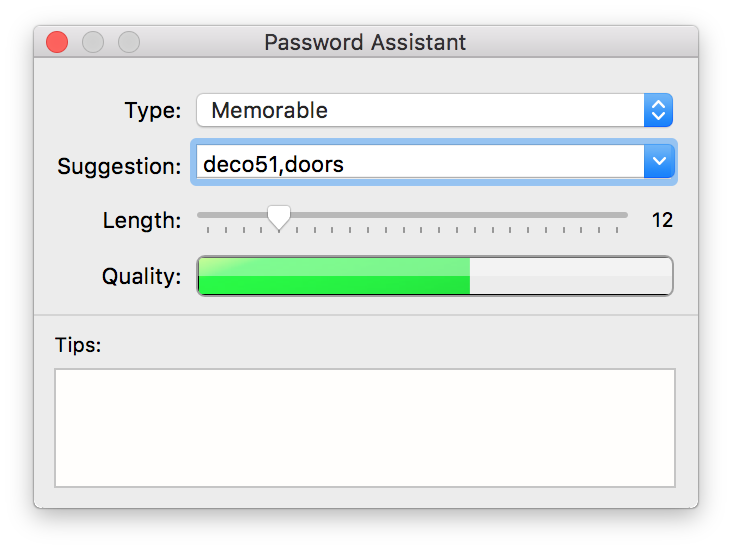
\includegraphics[width=0.49\linewidth]{rw/apple-pw-assistant-memorable}
		\caption{\label{fig:rw:pw_generators} On macOS, the Keychain application manages passwords for the user. If a new entry is manually created by the user, the password assistant can be used to generate different kinds of passwords: Random (image on the left), letters and numbers, numbers only, memorable (image on the right), and FIPS-181 compliant}
	\end{figure}
	% pseudo random 
	In the first paradigm, the generator creates pseudo-random strings resembling user-selected passwords. \textbf{Pronounceable} password generators do not yield random characters but random phonetic segments \cite{Gasser1975RandomWordPronouncable}. This allows users to repeat passwords in their head or saying them aloud to memorize them. However, generating passwords that are consistently pronounceable is challenging\cite{White2014IsntThatFabulous, Goldberg2015UnspeakablePasswords}. Passphrases can also be generated in the same way \cite{Kurzban1985Passphrases}. 
	% truly random
	The second option yields truly random character strings taken from an alphabet large enough to mitigate most guessing attacks (see example in Figure \ref{fig:rw:pw_generators}). Huh \etal propose letting users replace a certain number of characters to create a more memorable version of the random password \cite{Huha2015UserReplaceablePasswords}. However, memorization of random strings is still exceptionally tedious for most users, as is typing them. Therefore, such passwords need to be either be written down or stored inside a \gls{PWMg}. Most password managers (see Section \ref{sec:rw:external-storage}), offer to generate passwords. Moreover, the Safari browser suggests a randomly generated password to users and stores it into Apple's cloud storage Keychain. 
	% Usability benefits
	Relying on a \gls{PWMg} gives users a number of usability benefits \cite{Yee2006Passpet}. As mentioned above, auto-fill reduces interaction times and recall problems. If passwords are generated on the fly, the effort to create passwords is removed. It is easy to generate unique passwords for each account and thwart phishing attacks, so the \gls{PWM} scales with the number of accounts. Some \glspl{PWM} give the users feedback to assess their overall protection level (see Chapters \ref{chap:mental_models_pwm} and \ref{chap:pwrm}). 
	% Usability drawbacks.
	On the downside, users become dependent on the \gls{PWM}, which makes it difficult to roam and use other devices. Even if users do not generate passwords, they lose muscle memory with auto-fill, so it is cognitively more challenging to log in manually.
	
	% research about PWMs
	HCI researchers have tried to solve these problems. Stobert and Biddle proposed VersiPass \cite{Stobert2014PWMThatDoesntRemember}. It uses graphical authentication and hints to avoid losing muscle memory, but it has not been empirically evaluated. Tapas is a decentralized password manager based on two-factor authentication, which was well received in two user studies \cite{McCarney2012Tapas, McCarney2013PWMThesis}. Yee's PassPet is a browser extension that lets users pick a ``pet name'' (label) for each website they have signed up for \cite{Yee2006Passpet}. The label is part of the password hashing and aims to increase both the security and memorability of the scheme, similar to the Password Multiplier system by Halderman \etal \cite{Halderman2005ConvenientPWM}. Fagan \etal investigated the reasons for (not) adopting a \gls{PWMg} \cite{Fagan2017UsersConsiderationsPWMs}. They found that users more prominently appreciate usability benefits. Those who do not use a \gls{PWM} distrusted the security, potentially due to a sub-par mental model. We can also hypothesize that many users want to stay independent and not give away control to a third party. 
	
	% summary.
	In summary, password managers aide users with password selection, and scaling the increasing number of accounts. Generated passwords are mostly a go-to method for more proficient, security-aware users who actively seek to strengthen their passwords as much as possible. While the academic research community has not been able to create \gls{PWM} solutions with widespread adoption, many commercial solutions exist. However, the adoption rates indicate that current systems have not been fully adapted to the masses. 
	
	% Drawbacks: Single point of failure, security problems\footurl{https://www.businesswire.com/news/home/20151006006149/en/Latest-Data-Breach-Spotlights-Identity-Restoration}{11.01.2018} 
	
	% Kamouflage does not solve usability problems but is focused on security \cite{Bojinov2010KamouflagePWM}

	%%%%%
	%%%%%
	%%%%%	PERSUASIVE INTERVENTIONS
	%%%%%
	%%%%%
	\section{Persuasive Interventions}\label{sec:rw:persuasive-interventions}
	Persuading users to behave differently is the last line of attack we shall discuss in this part. Using technology to persuade users can be traced back to Fogg's seminal work on ``captology'', which was later recoined under the umbrella term \textit{persuasive technology} \cite{Fogg2002Persuasive}. He defines it as ``\textit{interactive computing system designed to change people's attitudes or behaviors}''. Persuasion itself is seen as ``an attempt to change attitudes or behaviors or both (without using coercion or deception)''. The latter part further distinguishes persuasion from manipulation, where people are not aware of the manipulator's intentions. Password composition policies exert authority and coerce users to follow the rules. The need for autonomy as part of the Self-determination theory \cite{Ryan2000SelfDeterminationTheory} is thus undermined by policies. User education is voluntary and misses its goal because users seldom decide to educate themselves on password security. Therefore, persuasion could fill the gap of providing transparent education by making alternative behavior more salient \cite{Forget2007PersuasionEducationSecurity}. In the context of this thesis, we thus understand persuasive technology as an \textit{enabling} technology that adequately supports users while respecting their preferences. Persuasion in HCI has become an essential topic with numerous papers published at top-tier conferences. Hekler already highlighted the rising interest already in 2013 \cite{Hekler2013TheoreticalGap}. What is more, persuasion is one of the central topics among the top-5 most cited CHI-papers of the past five years\footurl{https://scholar.google.com/citations?&view_op=list_hcore&venue=6NNnGOq9_mAJ.2017}{17.01.2018}. Consequently, we regard it as highly promising direction for password research. 
	
	\subsection{Background}
	In the following, we explore how to use persuasion to create ``soft paternalistic interventions that nudge users toward more beneficial choices'' \cite{Acquisti2017NudgesPrivacySecurity}.
	\todo{line of thought not consistent enough.}
	
	\subsubsection{Terminology in Persuasion and Behavioral Economics}
	In the design of persuasive technology, we often encounter the concept of ``nudging'' people, i.e. figuratively giving them a small push to act in a certain way \cite{Thaler2008Nudge}. The ``choice architect'' decides on the direction of the push \cite{Thaler2010ChoiceArchitecture}. For instance, by setting clever \textit{defaults}, people are relieved of making an active decision and can just accept the default. Nudging strategies as part of ``soft paternalism'' or ``libertarian paternalism'' stem from the field of behavioral economics, which studies ``how individual, social, cognitive, and emotional biases influence economic decisions'' \cite{Acquisti2008DigitalPrivacy}. In other words, behavioral economists embrace the idea that people sometimes act irrationally when making economic decisions. For example, people are significantly more likely to purchase a glass of jam, if there are only six options instead of 24 -- the so-called ``choice paradox'' \cite{Iyengar2000WhenChoiceIsDemotivating}. As we have seen in Section \ref{sec:rw:user-behavior}, password coping strategies ultimately involve such economic decisions: Given a risk, one needs to assess the severity, likelihood, costs of mitigating the risk, and the effectiveness of the protective measure \cite{Schneier2008PsychologySecurity}. Thus, theories from behavioral economics are a useful resource that can explain user behavior. 
	
	% where does irrational behavior come from? todo: is this part of terminology?
	Referring to the dual process theory, Kahneman argues that many sub-optimal decisions originate from System 1 which is responsible for intuitive and automatic thinking processes \cite{Kahnemann2002}. System 2, on the other hand, is the rational and effortful part in our thinking processes. He explains that most of our thinking is carried out by System 1, because it would be impossible to put the same amount of effort into every decision that we make (e.g. it is unnecessary to weigh the pro's and con's in answering ``should I brush my teeth today?'').  In Password selection, both systems are involved, but depending on the context, one or the other is primarily responsible for the decision. For instance, users who have formed the habit to reuse one password for all accounts will do the same for the next account they create, thus the automatic System 1 is at play. However, if the composition policy forces the user to modify their password, the cognitive challenge rises and activates System 2. Persuasive technology aims to either facilitate decision-making (i.e. supporting System 1), or block automatic processes to help the user adopt a different behavior (i.e. activating System 2). For instance, intentionally introducing delays during password authentication \cite{Malkin2013Waiting} or in browser warnings \cite{Egelman2010PleaseContinueToHold} lead to users spending more time on the task and act more securely, probably because the time was enough to activate System 2.  

	% examples for irrational decisions
	% how does persuasion help here?
	\subsubsection{Cognitive Illusions, Biases, and Heuristics}
	Irrational decision-making, according to behavioral economics, shows patterns around \textit{cognitive illusions} (also ``cognitive distortions'') and \textit{biases} \cite{Lockton2012CognitiveBiases}. Acquisiti \etal describe them as ``
	systematic, and therefore predictable deviations from rational choice theory'' \cite{Acquisti2017NudgesPrivacySecurity}. The resulting behavior is neither erratic, nor irrational, but may strongly influence judgment under uncertainty \cite{Tversky1974HeuristicsBiases}. To still be able to make decisions under uncertainty, people utilize \textit{heuristics}, or mental shortcuts in decision-making. \textit{Bounded rationality} explains the use of heuristics with the impracticality of assessing all possible options and outcomes. In other words, heuristics allow making good decisions under the circumstances \cite{Kahneman2003MapsOfBoundedRationality}. Thus, like biases, heuristics are not necessarily bad, but even necessary to get through life \cite{Cialdini2007Influence}.
	% cybersecurity entails uncertainty (``what's best for me?'')
	The lack of certainty is prevalent in decisions in cybersecurity, especially for mainstream users. For example, it is hard for users to assess the risk of threats online, and make a decision on the required protection level. Therefore, heuristics in this domain have been investigated to better understand user behavior. 
	% hey, let's look at a few examples.
	The list of cognitive fallacies is long, Wikipedia mentions 109 decision-making biases alone \footurl{https://en.wikipedia.org/wiki/List_of_cognitive_biases}{17.01.2018} (see Figure \ref{fig:rw:cognitive-biases}). Let us discuss notable examples that directly relate to cybersecurity\footnote{Please refer to Acquisiti \etal \cite{Acquisti2017NudgesPrivacySecurity} for an in-depth and highly valuable discussion of biases in privacy and security}. To stay on topic, we explain all effects with ``password phenomena'', although the scenarios have not necessarily been empirically substantiated.
	
	\begin{figure}
		\centering
		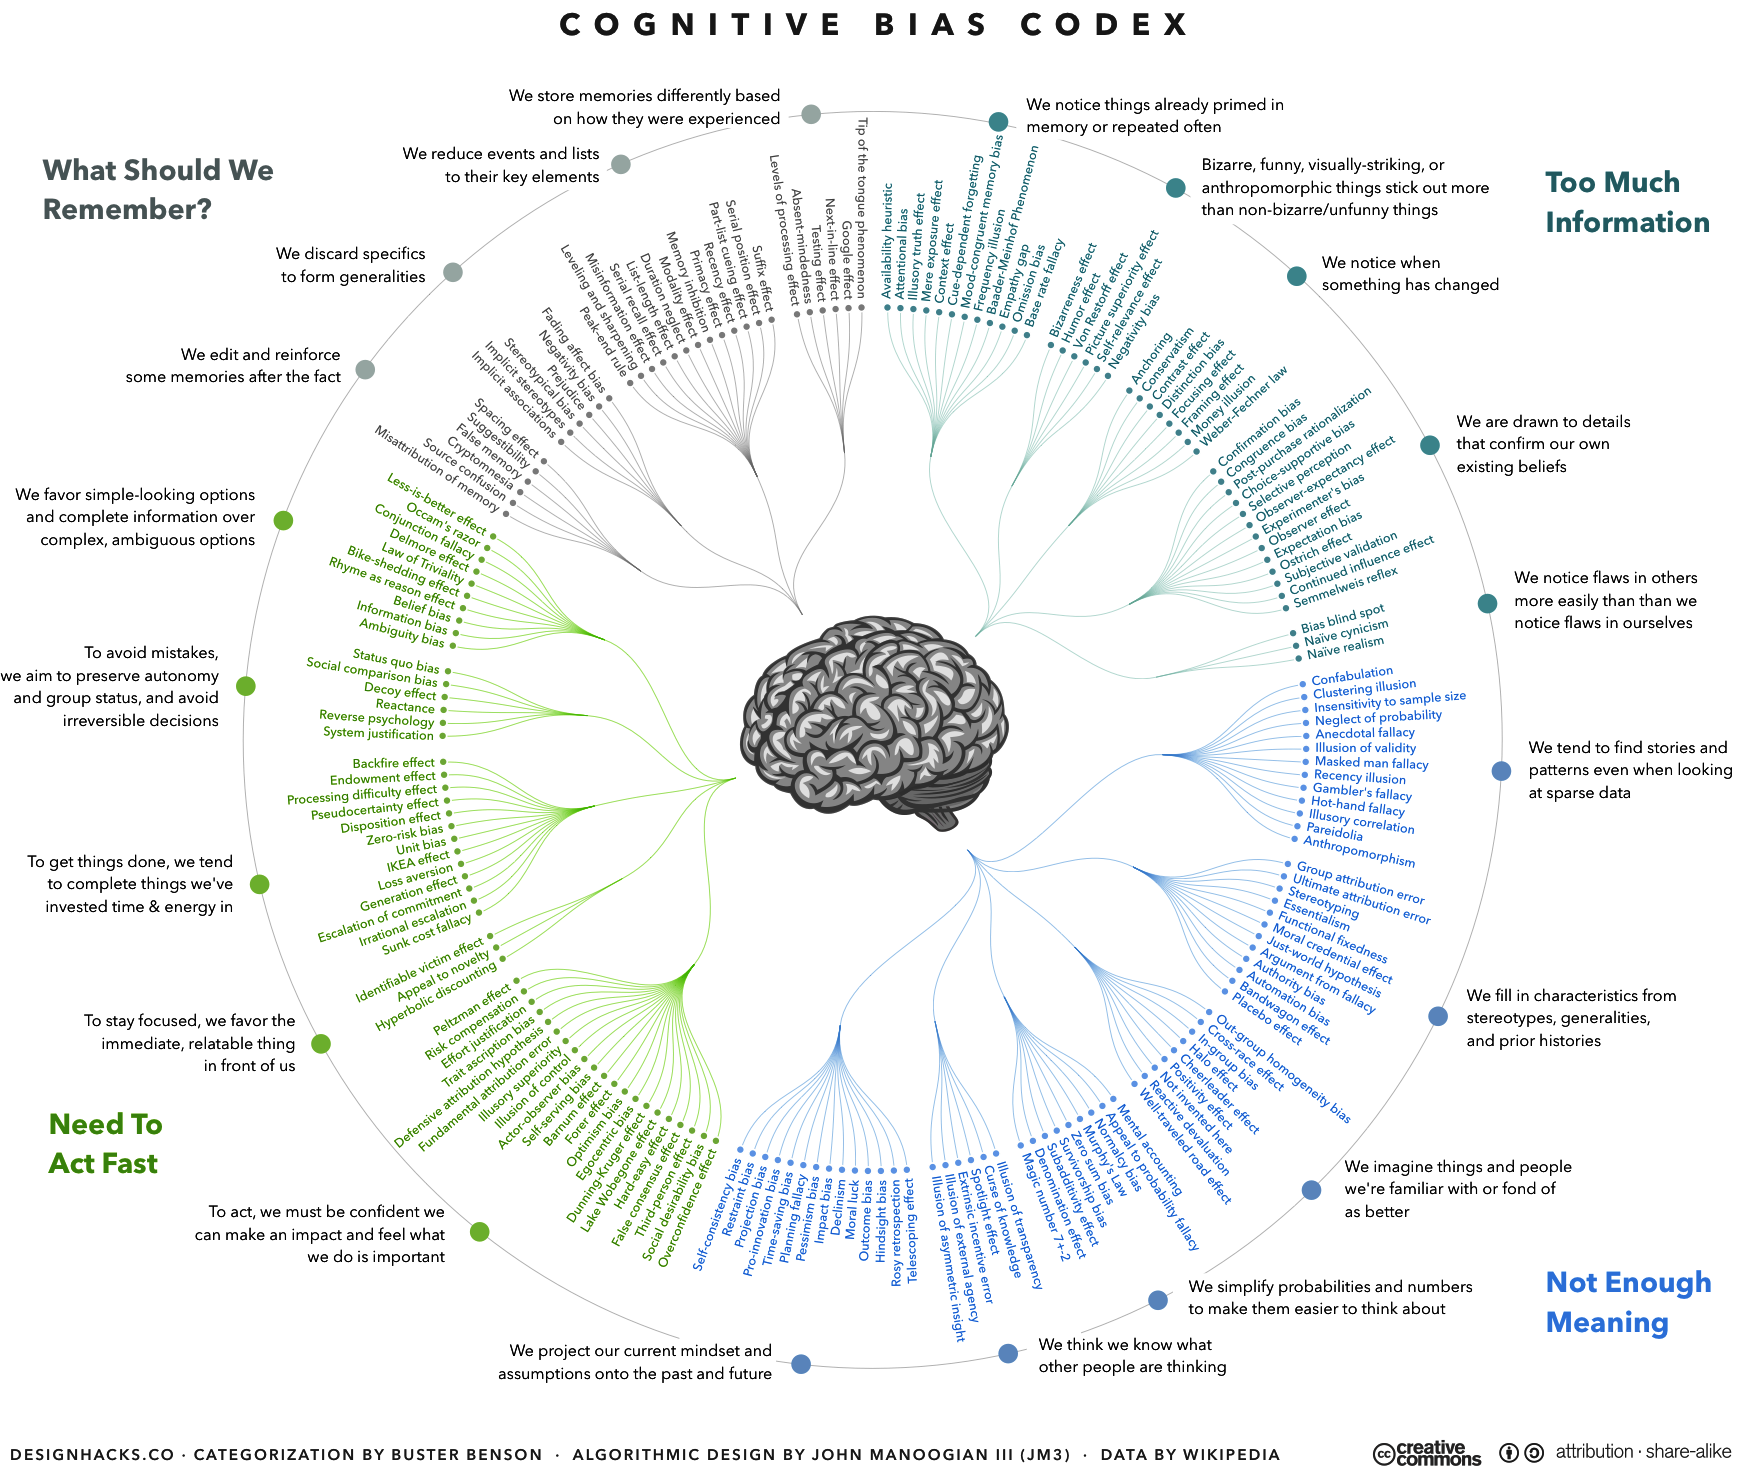
\includegraphics[width=1\linewidth]{rw/cognitive_bias_codex}
		\caption{\label{fig:rw:cognitive-biases}Categorization and visualization of cognitive biases listed on Wikipedia. CC-BY-SA Buster Benson, John Manoogian III}
	\end{figure}

	% sunk costs / disposition effect.
	The \textbf{sunk costs} fallacy describes the situation when people have made an investment under uncertainty in the past and continue to stand by it, even if circumstances have changed and it would be better to abandon the commitment \cite{Thaler2004MentalAccounting}: Imagine someone bought a (nonrefundable) ticket to watch a movie at a theater. They dislike it from the start and after 25 minutes, they feel the movie is not going to get better. Due to the sunk costs of the ticket and unrecoverable effort to go to the theater, it is likely that they stick around instead of simply leaving the show. Herley \etal hint a similar scenario for replacing password authentication \cite{Herley2012PersistenceOfPasswords}. In their point of view, \glspl{SP} have invested into passwords and are now reluctant to move away to alternative schemes, although they might improve system security (see Section \ref{sec:rw:authentication_without_pws}). Similarly, users who have committed to a password and reused it many times, might see the time spent as sunk cost. Thus, they do not switch to a more secure alternative even if they know there are plenty. Arguably, the \textbf{Status Quo bias} plays a role in both examples, too: people tend to favor a pre-existing state of affairs over potentially uncertain changes.
	
	%availability
	The \textbf{availability heuristic} is observed when people over- or underestimate the likelihood of events after being exposed to salient information. For instance, users might estimate the likelihood of being hacked as higher after someone in their social circle reports such an incident: the possibility has become more salient and available, thus future occurrences are seen as more probable. Das \etal partially confirmed such behavior through user interviews \cite{Das2014EffectSocialInfluenceSecuritySensitivity}. Certainly, \textbf{recency illusions} amplify the availability heuristic, i.e. a user who just found out about the ``hacking threat'' might think that this threat had just emerged. Such \textbf{salience} can be found at pass  % there are more examples in the same vein: frequency bias, selective attention/perception. 
	
	% anchoring and bandwagon.
	The \textbf{anchoring} bias creates reference points (or baselines) for decisions, especially comparisons \cite{Forget2007PersuasionEducationSecurity}. After a password breach, media reports typically mention some of the most-used passwords. Readers of news article anchor on the strength of obvious passwords like 12345 and compare their own. In many cases, their own password(s) seem much stronger by comparison, but might not be seen as strong if assessed separately. Similarly, if many people show insecure password behavior, this may reinforce an individual's practices through the \textbf{bandwagon effect}: ``if so many people behave insecurely, why would I act differently?'' \cite{Adams2015MindlessComputing}.
	
	% framing effects, preference reversal, loss aversion
	People can also be biased by the way information is presented, which is known as \textbf{framing effect} \cite{Verendel2008ProspectTheorySecurity}. The wording is key here and can generate \textbf{preference reversal} and other inconsistencies \cite{Huber1982AsymetricallyDominated}.  For password authentication, framing can be found in educating users about passwords. Zakaria \etal \cite{Zakaria2013DesigningEffectiveSecurityMessages} suggest instructing users through real-world security comparisons. Framing consequences for users around losses may trigger \textbf{loss aversion} -- a tendency to perceive losses as more valuable than equivalent gains \cite{Ariely2005LossesGains}. Garg and Camp argue that security is currently framed as a \textit{definite} loss for end users, while ``the risk of not investing in security is a \textit{probable}'', thus uncertain, loss \cite{Garg2013HeuristicsAndBiases}. Cialidini shows the importance of crafting \textit{normative} messages, that refrain from emphasizing that a socially unacceptable behavior is still widespread \cite{Cialdini2003CraftingNormativeMessages}. For instance, a normative message after a policy rejects the user's first-chosen password might explain: ``The password is weak, because it is easily guessable for hackers'' (emphasis on the adversary) rather than ``..., because it is something many people would choose'' (emphasis on the social in-group). If normative messages are framed badly, this can lead to the \textbf{backfire effect}, i.e. people behaving in the opposite way as intended. Thus, Weirich and Sasse see framing the attacker effectively as important opportunity in for persuasive password education \cite{Weirich2001PrettyGoodPersuasion,Weirich2005PersuasivePasswordSecurity}.
	
	% goal gradient effect
	As a final example of behavioral biases, people's motivation increases as they get closer to finishing a task. Hull coined this behavior the ``\textbf{goal-gradient hypothesis}'' \cite{Kivetz2006GoalGradient}. Behavioral economists have found it to induce irrational behavior: Kivetz \etal handed out two different designs of ``coffee cards'', that customers can fill up with each purchase \cite{Kivetz2006GoalGradient}. Once the card is full, they can redeem it for a free coffee. One of the designs had ten stamp-fields, while the other had twelve fields, two of which were already stamped. So, in both cases, customers received a free coffee after ten purchases. Surprisingly, more cards with twelve fields were redeemed after the trial period. People (wrongly) thought to be closer to goal, and thus were more motivated to achieve it. This ``goal distance model'' is sometimes used by password meters, i.e. a visualization of password strength (we discuss them in great detail in Section \ref{sec:rw:password-meters}). Password strength visualization can give the user a ``head start'' to motivate them to fill up the entire bar and achieve a ``strong password'' (i.e. a full loyalty card). 
	
	% overconfidence
	% hyperbolic discounting
	%immediate payoff: get access to account now. Make choices today that future selves would not have made despite the same level of information
	%IKEA effect: people put disproportionally more value on objects partially built themselves. a suggested password might not be suitable, because it lacks ``personal effort''. Huh \etal leverage the IKEA effect by letting users replace characters of generated passwords. 	
	%Ostrich effect occurs when people ignore an obvious negative situation. Users who know that 

	%Choice proliferation / choice paradox \cite{Knijnenburg2013MorePrivacyOptions,Korff2014TooMuchChoice}

	% automation bias
	% potentially helpful if time allows: 
	% Bellur2014HeuristicsUsed

	\subsection{Persuasive Design Patterns in Usable Security and Privacy}\label{sec:rw:persuasive_patterns}
	Phenomena involving biases and heuristics are often directly translated into a persuasive strategy. It is interesting that apparently the lines are blurred between the two concepts. Anders Toxboe collected a number of persuasive design patterns on his website\footurl{http://ui-patterns.com/patterns}{21.01.2018}, which highlights this blend of psychology and persuasion. There is, however, no such list for patterns specifically for interventions in usable security and privacy. Therefore, we start with the discussion of general frameworks and put them into the context of security and passwords.
	
	\subsubsection{General Frameworks}
	\gls{PD} has been tried to formalize in several frameworks. Fogg's Behavior Model posits that three elements must converge to achieve a target \textbf{B}ehavior: \textbf{m}otivation, \textbf{a}bility, and \textbf{t}riggers (B=mat) \cite{Fogg2009BehavioralModel}. For passwords, this implies that people need to be motivated to protect themselves, at the same time the need to know how to achieve protection and be exposed to a trigger. Triggers work best when presented at the \textit{opportune moment} (or ) \cite{Lockton2010DesignWithIntent}.  % The trigger is perhaps the most interesting part for persuasive design in the realm of authentication, because 
	Lockton \etal proposed the ``Design with Intent'' framework as a toolkit for persuasive interventions \cite{Lockton2010DesignWithIntent}. Jameson \etal show how to pick strategies from various toolkits to create a persuasive choice architecture \cite{Jameson2011PreferentialChoice}. 
	% example walk through on a generic level
	Cialdini's generic ``\textbf{six weapons of influence}'' have been used in the design of persuasive technology \cite{Cialdini2007Influence}. He lists authority, scarcity, liking, social proof, commitment \& consistency, and reciprocity as the principles of persuasion. Let us walk through their potential usage in password authentication. 
	% authority
	The authority principle says that people are likely to follow the instructions of an authority, which explains why the \gls{NIST} guidelines have been widely adopted despite their downsides. 
	% scarcity
	Scarcity drives motivation to act quickly to avoid losing an opportunity (see loss aversion), and framing effects are used to communicate the scarcity of a resource. For instance, the ``419 scam'' tactic in phishing emails frames time as a scarce resource: ``your account has been intruded, if you don't log in now, you lose access to it permanently'' \cite{Stajano2011Principles}. In this case, persuasion is used for malicious purposes. 
	% liking
	People prefer to comply if they \textit{like} their counterpart. In theory, this would make password requirements less bothersome if used on a website that users like, or in a more aesthetically pleasing way. Although there is no empirical evidence that the principle works for registration forms specifically, other HCI research points in this direction \cite{Tractinsky2000WhatIsBeautiful, Fogg2001WhatMakesSitesCredible}. %TODO run a micro-survey to explore this, that's interesting. 
	% social proof
	The social proof strategy makes other people's behavior more \textit{available} because in decision-making people tend to copy others' decisions. For instance, it might help to point out that millions of users are already using a password manager in a news article about a new password leak. We can also apply Fogg's behavior model here: Reading about a password leak \textit{motivates} users to protect themselves, the social proof strategy acts as a \textit{trigger}, and mentioning the ease-of-use of password managers gives users confidence about their ability to adopt a \gls{PWM}. 
	% commitment & consistency
	The commitment \& consistency principle is an immediate part of the Password Life Cycle \cite{Stobert2014PasswordLifeCycle}. People try to be consistent with their past behavior and their past values. Thus, a small step towards breaking an insecure habit might, in fact, induce more secure behavior afterward. If a policy forced a user to stop using a common password, the effort to commit to the new password might spread over to other accounts, too. Stobert found that cybersecurity experts show higher signs of consistency \cite{Stobert2015ExpertPassword}. Thus, if another persuasive strategy achieves that users commit to a new password selection scheme, their behavior might become more consistent and thus be elevated to the expert level. 
	% reciprocity
	Finally, reciprocity describes the desire to return a favor. To use it as a persuasive design strategy, one has to do something favorable for the users first. Thus, offering users to store their passwords in a secure place and automatically logging them in is a good foundation to ask them later to turn on 2-factor authentication to help secure their account.
	
	\subsubsection{The Persuasive Authentication Framework (PAF) by Forget \etal}
	Forget \etal embraced persuasion as technique to help users act more securely in password authentication \cite{Forget2007PersuasionEducationSecurity}. In 2007, the put forward the \gls{PAF}, which breaks down the dimensions of persuasive design specifically for password support systems. In the following we describe it on a high level and illustrate its components with results from empirical studies. 
	
	\begin{figure}
		\centering
		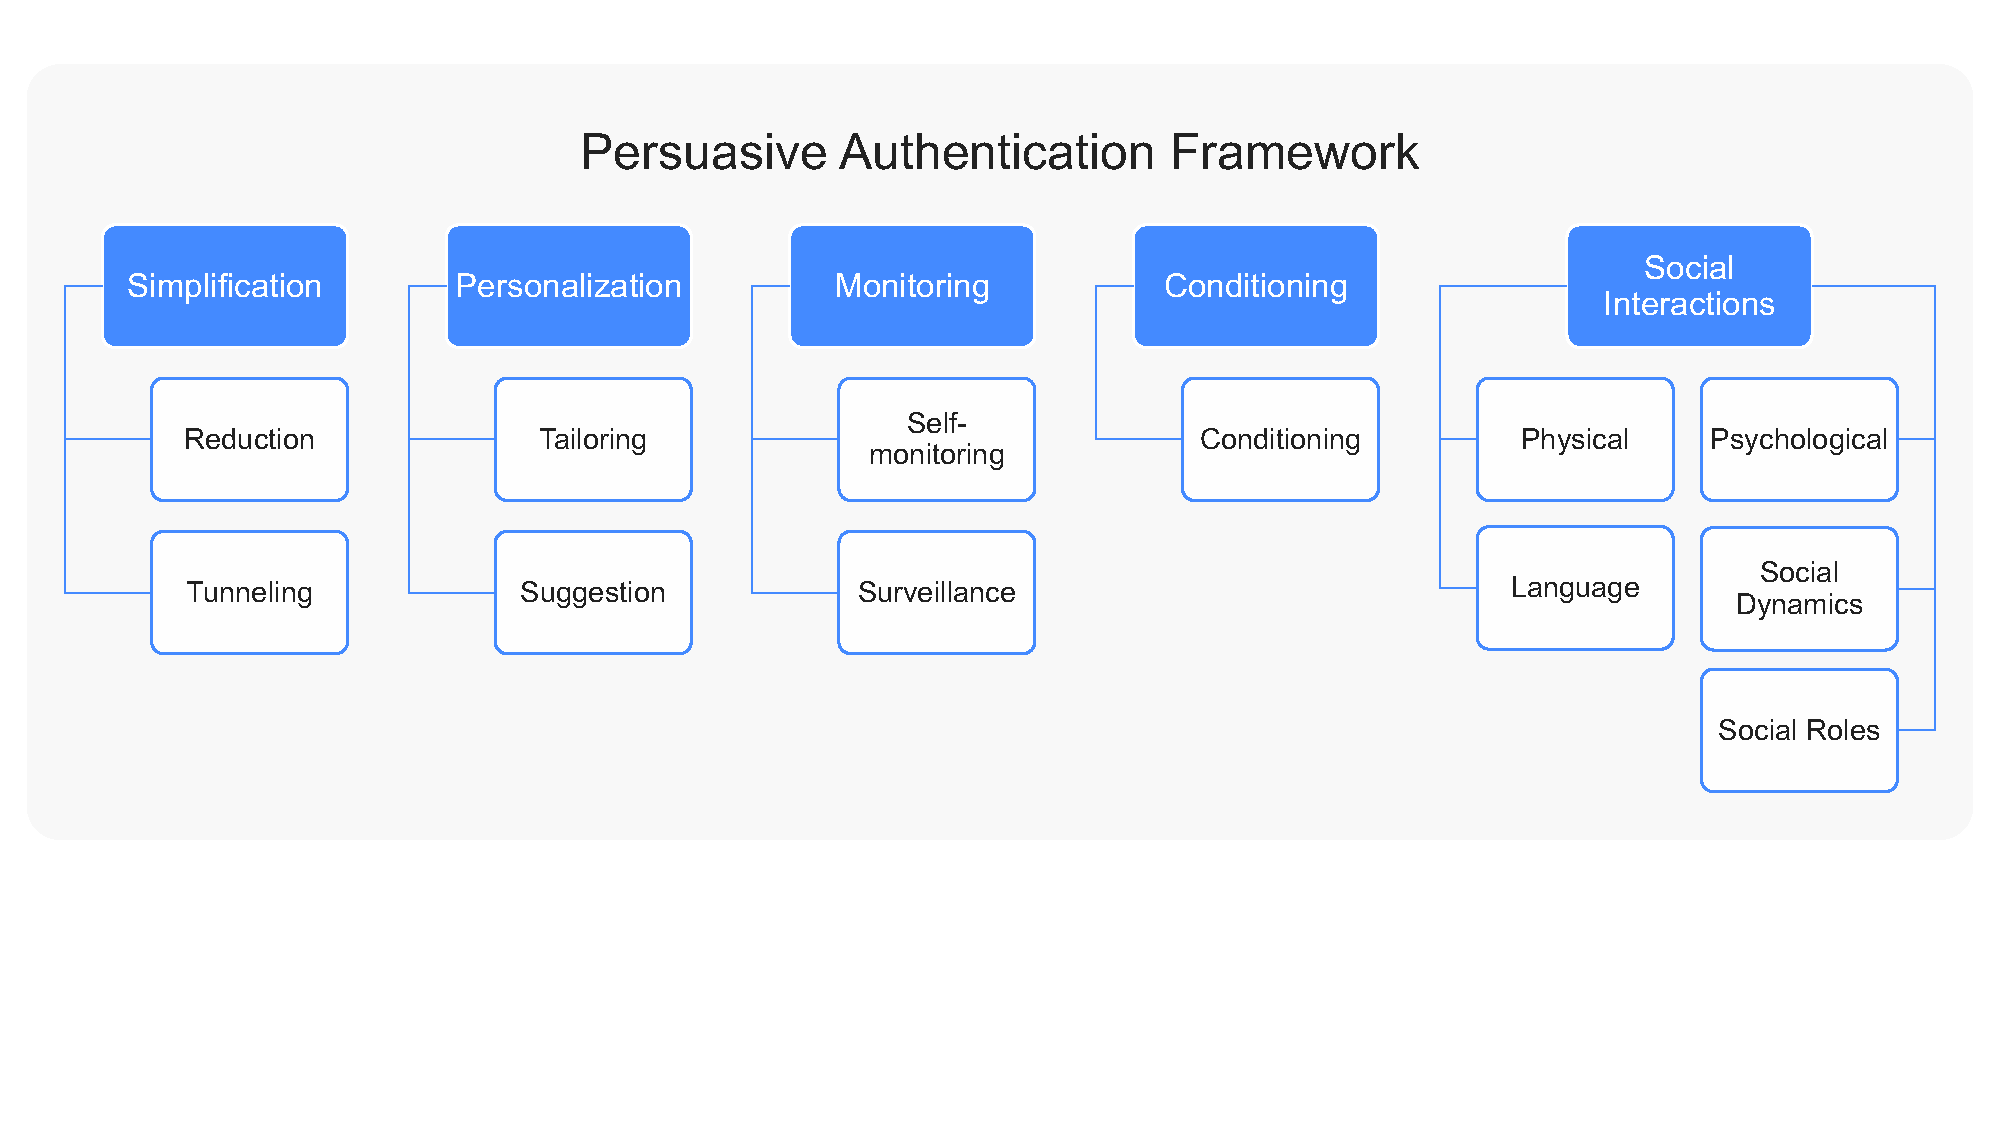
\includegraphics[width=\linewidth]{rw/paf}
		\caption{\label{fig:rw:paf} Elements of the persuasive authentication framework.}
	\end{figure}

	%simplification
	The \textit{simplification} principle posits to reduce the number of tasks to achieve an overall goal. Thus, the hypothetical distance between start state and goal is shorter, so, goal-gradient effects become visible. Password managers usually simplify authentication by reducing the best-case interaction from Recall-Enter-Submit to Submit. Fagan \etal showed that simplification is the primary reason to adopt a password manager \cite{Fagan2017UsersConsiderationsPWMs}. But even without a \gls{PWM}, both the ``recall'' and the ``enter'' sub-tasks can be simplified. Recall is facilitated with consistent password strategies. Entering is easier the primary password is replaced by a less complex one-time password. 
	
	% Personalization:
	\textit{Personalization}, as understood in the \gls{PAF}, encompasses tailoring the experience to an individual user, or to suggest actions. 
	% tailoring / individualization
	A recently (\ar) emerged design pattern spreads out the log-in process across two separate steps for username and password, rather than having the two input fields visible at once. After submitting the username, the page is \textit{tailored} to the user by showing them their profile picture and/or another piece of non-critical personal information. At the same time, this establishes a light-weight trusted path \cite{Ye2005TrustedPaths}. Wilkinson \etal suggest personalizing privacy by design by giving users different levels of control to depending on their privacy profile \cite{Wilkinson2017UserTailoredPBD}. Besides, this is a good example of the paternalism in persuasive interventions, because the designer what option is ``better'' for the individual user. Similarly, it is conceivable to personalize password policies depending on the user's ``password profile'' (see \ref{sec:pst:personalizing-policies}). Moreover, personality constructs have been investigated to tailor user experiences, which perhaps exceeds the original proposition in the \gls{PAF}. Recently, Egelman and Peer advocated the use of psychometric cues to contextualize privacy or security messaging, which they call the ``next frontier in privacy and security research'' \cite{Egelman2015AverageUser}. Jeske \etal investigated user profiles for the susceptibility to security nudges \cite{Jeske2014NudgingWhomHow}. In their experiment, they used \textit{salience} to steer users away from insecure wireless networks. They found that participants with low impulse control were more susceptible to nudges. The finding can be interpreted that nudges directed at System 1 seem more effective. There is also preliminary evidence that susceptibility to phishing, i.e. a social nudge, is also related to personality \cite{Halevi2013PilotStudyPersonality}. It stands to reason that password selection is related to personality, too (see Chapter \ref{chap:pws_and_personality}). If this were the case, a new spectrum of personalization strategies arises. Haque \etal have already proposed a psychometric construct to identify such associations \cite{Haque2014PsychometricsStrongPassword}.
	% suggestion
	Forget \etal list \textit{suggestion} as part of the personalization dimension, because suggestions might be based on a personal context factors. They provided a number of cases studies on suggestive password alterations \cite{Forget2008ImprovingPasswordsThroughPersuasion, Forget2008MemorabilityPersuasivePasswords, Forget2008PersuasionStrongerPasswords}. The ``persuasive text passwords'' (PTP) system takes a user's password and either randomly inserts characters or replaces existing characters to increase strength. The high resemblance to the original password is supposed to maintain memorability \cite{Forget2008MemorabilityPersuasivePasswords}. Shay \etal later re-evaluated the approach in an MTurk study, which yielded mixed results \cite{Shay2015SpoonfulOfSugar}. 
	
	
	% monitoring
	Arguably, observing what users do increases the chances that they comply to security policies, given that users are aware of being observed. \textit{Monitoring}, however, can entail reduced user experience (cf. need for autonomy \cite{Ryan2000SelfDeterminationTheory}). Nevertheless, if used adequately, it can serve as \textit{authoritative} strategy (cf. Cialdini's six weapons of influence \cite{Cialdini2007Influence}). Google's password alert\footurl{https://github.com/google/password-alert}{20.01.2018} is a moderate approach to secure users' Google accounts. It is a browser extension that alerts the user if they type in the password of their Google account on unrelated web pages. Hence, the idea is to make sure users use a unique password for their Google account, which is a central hub for various services. To work properly, the browser extension needs to access every keystroke. Some users might distrust it because, although it is open source, it is hard for them to tell if their private data is collected. Prospect theory tells us that in this judgment under uncertainty, losing private data is attributed a higher value than the security gain. % not sure I want to bring have that argument. 
	A less privacy-invasive design element that might help in relieving uncertainty is \textit{self-monitoring}. Self-monitoring through \textit{feedback-loops} -- another design pattern \cite{Lidwell2003UniversalPrinciplesOfDesign} -- allows users to reflect on their past actions and derive alternatives to attain their goal. Some \glspl{PWM} create a ``security score'' for each user and persuade them to improve it (see Table \ref{tbl:pwrm:pwm_comparison} in Chapter \ref{chap:pwrm}). 
	
	% conditioning
	Users rarely develop habits to act securely. Thus, Forget \etal argue to use various forms of reinforcement to persuade people to develop such habits. Rewarding users for secure password behavior serves to \textit{condition} them. Google Drive, for instance, offered users more cloud storage quota if they completed a two-minute security check-up \footurl{https://twitter.com/googledrive/status/697104410296455168}{20.01.2018}. Positive feedback during password selection can condition users, too. Other rewards, e.g. longer session expiration or faster system response, have not seen significant uptake. 
	
	% social interactions
	Lastly, the \gls{PAF} includes \textit{social interactions} as persuasive design strategy. Forget \etal posit that authentication systems mimick, e.g., the users' language to convey ``team spirit'' \cite{Forget2008PersuasionStrongerPasswords}. Weirich and Sasse \cite{Weirich2001PrettyGoodPersuasion}, respectively Sasse and Flechais \cite{Sasse2005UsableSecurityPosition}, similarly describe authentication as \textit{socio-technical system} that follows a social protocol. DiGioia and Dourish formulated the \textit{social navigation} pattern \cite{DiGioia2005SocialNavigationUsableSecurity}. To perceive the system as capable communication partner, signs of previous interactions inspire trust. Egelman \etal tried to nudge users during password selection through the \textit{social proof} strategy \cite{Egelman2013DoesMyPasswordGoUpToEleven}. A visualization informed the study participants how well their password fared compared to other users, e.g. ``your password is stronger than that of 85\% of our users''. They did not find evidence that this persuasive strategy influenced people, but maybe the approach could have been more focused on the \textit{proof} aspect, rather than \textit{competition}. The normative message can be read as ``other people's passwords are bad, but many people act this way''. This could actually evoke backfire effects through social proof: although users see their password is stronger, they believe that the social norm is to pick weaker passwords, which makes them conform to the social norm. In fact, Weirich and Sasse have provided empirical evidence for such behavior \cite{Weirich2001PrettyGoodPersuasion}. Social interactions are perhaps one of the most powerful design elements to persuade users: Das \etal reported that radical behavior changes often occurred due to social processes \cite{Das2014EffectSocialInfluenceSecuritySensitivity}. They argue that it is critical for users to observe experts in their social circle to raise their awareness and motivation for cybersecurity. Thus, persuasive design could make expert behavior of known peers more visible
	
	% final words on PAF
	In a number of ways, some ideas from the \acrlong{PAF} were rather optimistic and from today's point of view they appear questionable (e.g. conditioning users like animals). Much evidence from the ten years that followed its publication shows that persuasion does not always work as intended, so maybe a few suggestions were a bit naive. Renaud \etal evaluated eight nudges that were supposed to make students create stronger passwords \cite{Renaud2017LessonsLearnedNudges}. They reached the disheartening conclusion that none of them work. Nevertheless, certain aspects have caught on and are actively used, like Google's Password Alert which is a direct implementation of Forget \etal's ideas. We can conclude that the \gls{PAF} has matured over time, with certain components receiving more weight through empirical evidence, and others becoming obsolete. Thus, a revision could incorporate our newly gained understanding of persuasive authentication.
	%%%%%%%%%%%%%%%%%%%%%%%%%%%%%%%%%%%%%%%%%%%%%%%%%%%%%%%%%%%%%%%%%%%%%%%%%%%%%%%%%%%%%%%%%%%%%%%
	
	\subsubsection{Dark Patterns}
	At the outset of this chapter, we discussed ethics as critical factor in password studies. Using persuasion inherently becomes ethically problematic if the intention of the influencer is concealed, either by poor design or by choice. Persuasive techniques are used to manipulate, too. Many social engineering scams  
	on malicious websites use persuasion techniques, too. Muscanell \etal investigated the misuse of Cialdini's weapons of influence in cyber scams \cite{Muscanell2014WeaponsMisused}. They found that scammers exploit all of them in social engineering attacks. Muscanell \etal also propose mitigation strategies, but do not lay them out in detail. Attacks that take advantage of ``scarcity'' as persuasive strategy often rely on \textit{fear appeals}, e.g. ``Your computer is infected, download this software \textit{now} to remove all threats''. Xu \etal proposed using similar fear appeals to nudge users towards anti-spyware measures \cite{Xu2007FearAppeals}, and Vance \etal utilized the ``time to crack'' as fear appeal during password selection \cite{Vance2013FearAppeals}. There are a number of ``dark patterns'', which Nodder dismantles in his book ``Evil by Design'' \cite{Nodder2013EvilByDesign}. Some of them are still benign, others highly manipulative. DarkPatterns.org summarizes them briefly, e.g. \textit{misdirection} - where the design aims to focus the user's attention on a decoy to plant something on them\footurl{https://darkpatterns.org/types-of-dark-pattern}{20.01.2017}. However, Sasse strongly urges to resist them in the design of password persuasion because they wear off over time and often exaggerate the risks \cite{Sasse2015ScaringBullying}. Hence, dark patterns most likely turn out counterproductive. 
	
	%%%%%%%%%%%%%%%%%
	%%%%%%%
	%%%%%%		PASSWORD METERS  	XXXXXXXXX XXXXXXXXX XXXXXXXXX --------- ---------
	%%%%%%
	%%%%%%%
	%%%%%%%%%%%%%%%%%
	\subsection{Password Meters: Persuasion at Play}\label{sec:rw:password-meters}
	The most prominent and widespread persuasive strategy directed at passwords are \gls{PSM}. Most commonly, they  proactively estimate the strength of a password at entry time and visualize it. Often, verbal feedback accompanies the visualization. They have been used on a multitude of websites, in password managers, and as standalone tools. When they are used on a website or in a \gls{PWM}, there are a number of persuasive patterns at play:\newline
	\textbf{Feedback} and \textbf{self monitoring}: Users are enabled to make an informed decision regarding the security of the password.
	\textbf{Kairos}: Meters are presented at the opportune moment of protecting an account.
	\textbf{Goal-gradient effect}: The closer users get to a password that is deemed strong the more motivated they become to achieve the strong rating.
	\textbf{Simplification}: A visual strength bar is universally understandable.
	\textbf{Personalization}: The dynamic visualization is user-dependent.
	\textbf{Suggestion}: Some meters suggest alterations if they detect weak passwords.
	\textbf{Reinforcement}: positive feedback about the user's password can reinforce secure behavior
	\textbf{Authority}: If the service provider is a trustworthy entity, their feedback is more likely to influence the selection 
	\textbf{Social interaction}: Verbal feedback can speak the user's own language and open a dialog. 
	\textbf{Loss aversion} and \textbf{scarcity}: The strength estimation is only shown during password entry -- an opportunity to learn about one's own abilities which should not be missed. 
	\textbf{Availability} and \textbf{salience}: The strength estimation makes weaknesses more salient and threats more available. 
	\textbf{Framing}: verbal feedback and color coding allow framing the strength in a nuanced way.
	
	% history
	Balancing all those strategies in a particular design has received much attention in HCI and security research. It is hard to trace back their origins, but proactive password checks have been part of policies since the late 1980s \cite{Wheeler2016zxcvbn}. Bishop and Klein developed the \texttt{pwcheck} command-line tool that was used to give terminal-users feedback on their password selection \cite{Bishop1995ProactivePasswordChecking}. A core challenge is the strength estimation proxy. Websites cannot implement a full-fledged cracking infrastructure just for the sake of password feedback. Thus, proxies and estimators are the go-to method. 
	
	% do they work or not?
	\subsubsection{Effective or not?}
	A number of studies have been conducted on the effectiveness of password meters. Ur \etal explored 14 different designs, respectively settings, of password meters \cite{Ur2012HowDoesYourPasswordMeasureUp}: different variations of the ``bar'' visualization, different stringency parameters, suggestions, and nudges. They were able to identify significant differences in passwords strength depending on the meter. Very stringent meters led to stronger passwords. Any kind of visual meter resulted in longer passwords, so text-only feedback is less persuasive. Many participants in their \gls{mTurk} study added another character at the end to receive a higher rating from the meter. Qualitative feedback and usability ratings showed that the stringent meters were unpleasant for many participants, reducing their persuasive power. Egelman \etal investigated context factors in the effectiveness of meters \cite{Egelman2013DoesMyPasswordGoUpToEleven}. They found that password meters seemed to have a greater positive effect on strength, if they were displayed on a site with higher perceived value. Participants in that study did not ``need'' the password meter, but receiving feedback on highly values websites made their importance more available. At the same time they concluded, that the design of the meter plays an insignificant role and that social nudges do not affect strength either. Moreover, both Ur \etal's and Egelman \etal's study showed that memorability was not affected by the meters.
	% the ``state of the art''
	The meter with the highest reported effects was recently presented by Ur \etal \cite{Ur2017DataDrivenPWMeter}. After carefully evaluating the design space for rhetorical framing of strength feedback \cite{Eargle2015YouCanDoBetter}, they isolated the components of password meters and compared their effectiveness. They found that textual feedback is recommendable to create more persuasive meters. However, the policy affects the effectiveness, too. Their final design (see Figure \ref{fig:rw:cups-meter}) uses a number of persuasive elements: A visual bar to simplify communicating password strength; text feedback about the strength; explanations about the scoring with clear calls to action (tunneling strategy); and lastly, a personalized suggestion of an alternative password. 
		
	\begin{figure}
		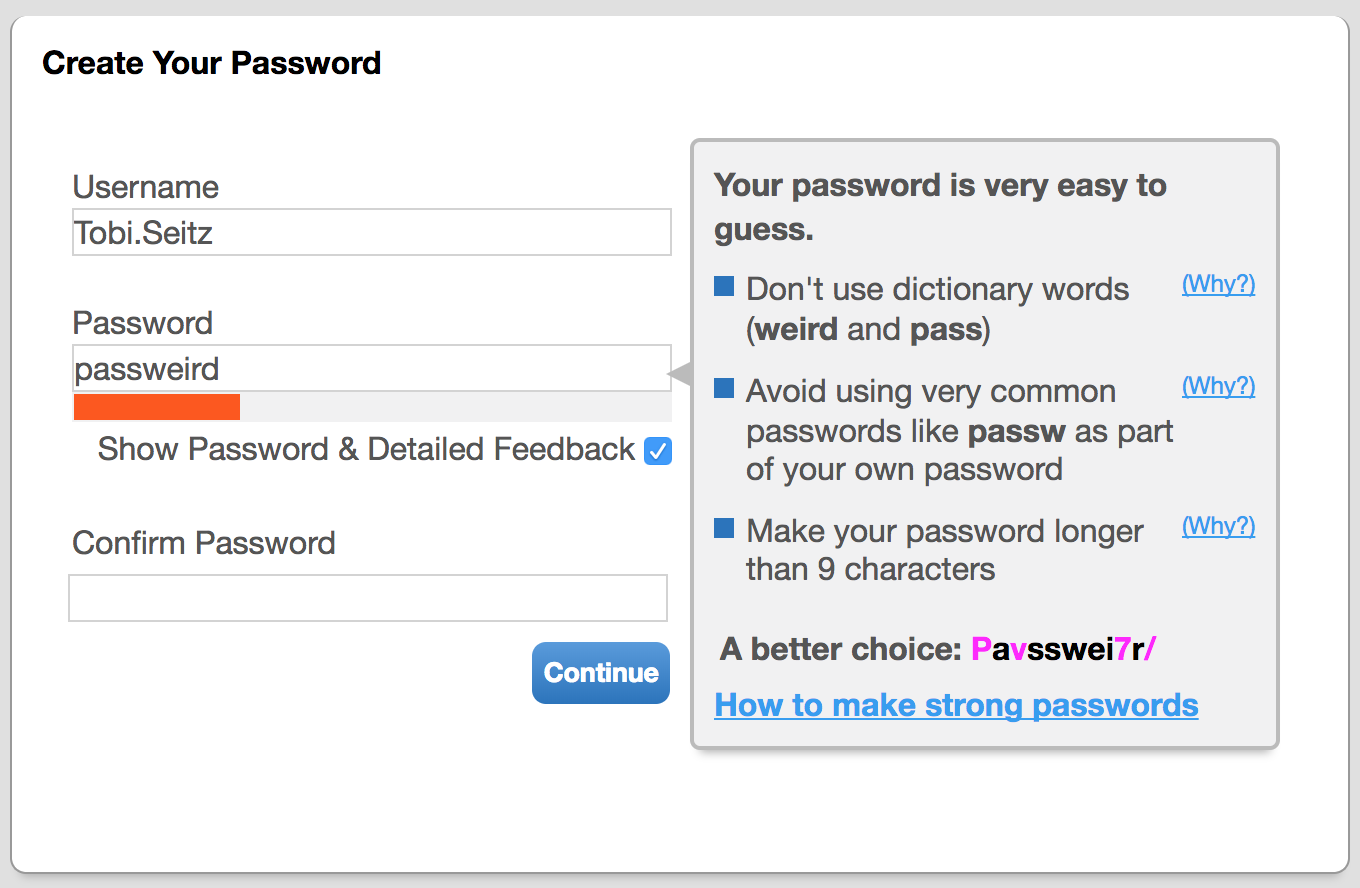
\includegraphics[width=0.49\linewidth]{rw/cups-meter-1}
		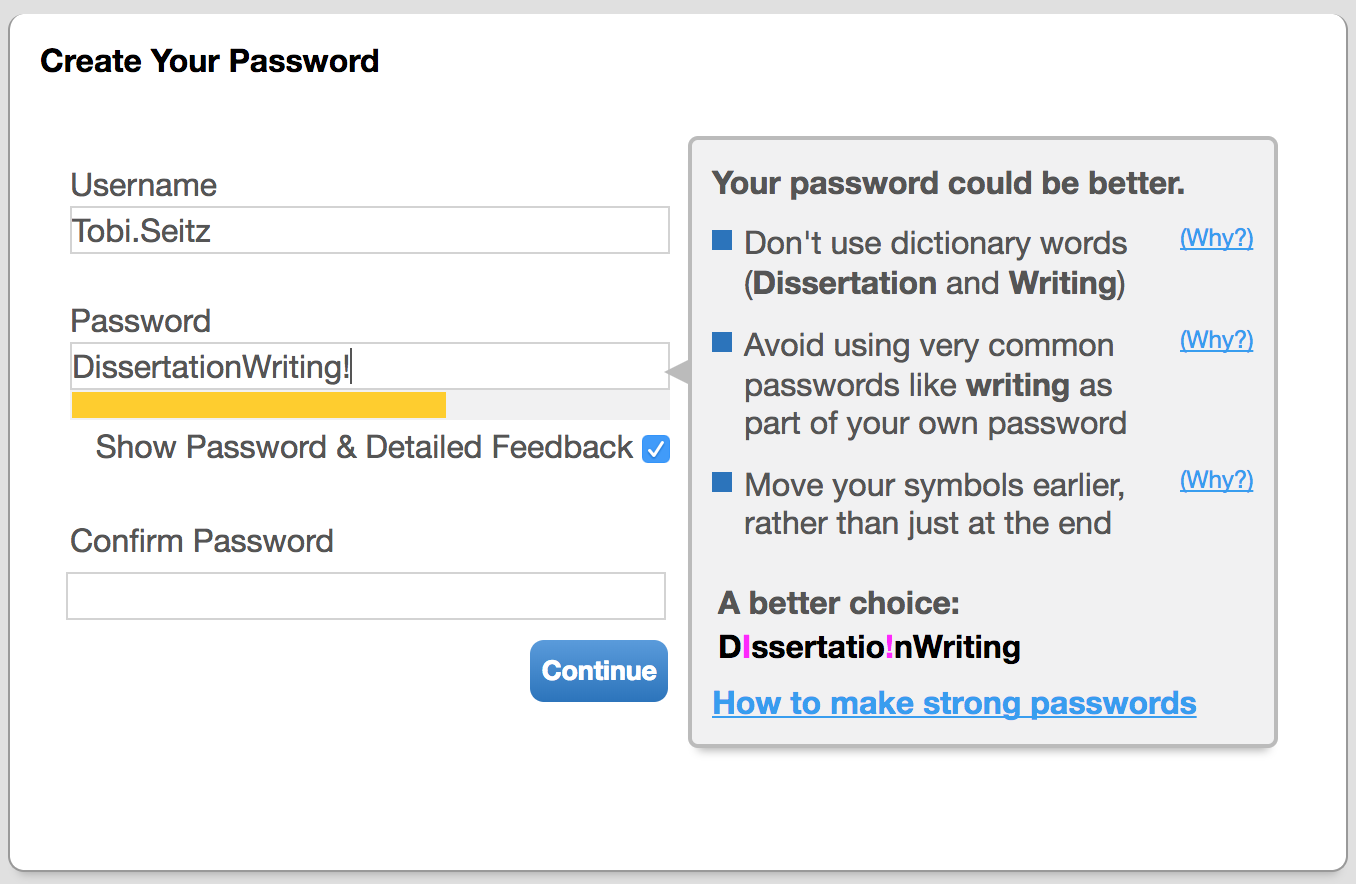
\includegraphics[width=0.49\linewidth]{rw/cups-meter-2}
		\caption{\label{fig:rw:cups-meter}}
	\end{figure}
	
	% novel ideas for password meters.
	\subsubsection{Beyond colorful bars}
	% telepathwords
	Visualizing strength is not the only way to design a password meter. Komanduri \etal crafted a sly prototype to tell users their passwords are predictable: their \textit{Telepathwords} system predicts the next character the user is about to type \cite{Komanduri2014Telepathwords}. The rationale of the system is that users do not mindlessly enter a weak password anymore, i.e. that the feedback should activate System 2 thinking processes. Furthermore, realizing that the next character can be automatically guessed might evoke fear appeal and steer people away from predictable passwords. Komanduri \etal evaluated Telepathwords with an \gls{mTurk}-study using a role-playing scenario. They found that password created in the Telepathwords groups outperformed traditional password policies in regard to strength and memorability. However, participants were significantly more annoyed by Telepathwords, perhaps because of the inconvenient truth and fear appeal. 
	% fear appeal and context info
	Communicating password strength with background information is another technique to persuade users. For example, Yee \etal displayed the estimated \textit{time-to-crack} when users selected a master password for the PassPet \gls{PWMg} \cite{Yee2006Passpet}. For users, it is much easier to translate this metric into a behavior than a numeric score like ``3/5''. Vance \etal found that such fear-appeal strategies persuade users to read password advice and modify weak passwords \cite{Vance2013FearAppeals}. Khern-am-nuai \etal also measured the persuasiveness of context-based warning messages as part of the password meter \cite{Khern-am-nuai2017ContextBasedMeter}. They found that participants in their \gls{mTurk}-study made significantly more changes to their initial choice when a warning was present, e.g. ``Weak. We estimate
	that the password you chose is among the 30,000 weakest passwords''. However, the study suffered from a few important limitations (e.g. removing all data from users who were unable to log-in after 30 to 60 minutes). 
	% different visualizations	
	Kroeze and Olivier proposed evolving a Pokemon figure as users type to visualize the growth in strength  \cite{Kroeze2012GamifyingAuthentication}. Furnell and Esmael evaluated feedback through emojis and found positive effects on the length of user-selected passwords \cite{Furnell2017GuidanceCompliance}. Afjan \etal allowed users to interactively explore the visualization they had received from the password meter \cite{Aljaffan2017PasswordSecurityVisualizer}. Ur \etal report that a dancing bunny animation that dances faster with increasing strength failed to nudge users better than less exciting meters \cite{Ur2012HowDoesYourPasswordMeasureUp}. Shay \etal tried to help users select a stronger password through a wizard that explained mnemonic phrase-based passwords \cite{Shay2015SpoonfulOfSugar}. Besides, they compared this strategy to the insertion approach we saw in Forget \etal's persuasive text passwords (PTP) \cite{Forget2008ImprovingPasswordsThroughPersuasion}. Both approaches were generally disliked by the participants, though. 
	
	% a different kind of meter: guidance makes policies less annoying / assistance / suggestion
	Apart from pure strength visualization and persuasive messages, real-time feedback can accompany a password policy. The user sees a list of requirements and as they enter their password, they get feedback on the aspects that have already been fulfilled, which was originally proposed by Proctor \etal \cite{Proctor2002ImprovingAuthenticationProactivePasswordRestrictions}. Although we know by now that the resulting passwords are not necessarily stronger, Shay \etal found that this kind of checklist can reduce user frustration with policies in general \cite{Shay2015SpoonfulOfSugar}. Feedback is also crucial if the policy utilizes blacklists to ban too easily guessed passwords \cite{Shay2014CanLongPasswordsBeSecureAndUsable}. Habib \etal evaluated Ur \etal's data driven password meter for situations where blacklists are present \cite{Habib2017Blacklists}. They found that text feedback mitigates insecure selection especially for those users who intended to use a blacklisted password. 

	% summary
	\subsubsection{Light and Shadow}
	Evidence about the effectiveness of password meters is mixed, but Ur \etal's strategy might be one of the most persuasive ones, because it combines many techniques that have proven successful in different areas of persuasion \cite{Ur2017DataDrivenPWMeter}. So, in certain contexts, password meters can definitely nudge users towards more secure behavior. 
	
	However, where there is light, there is also shadow. Meters influence users' mental models of password strength in similar ways as policies. However, as with policies, it is near impossible to reach consensus on all parameters of pro-active measures and metrics for all contexts. 
	% real word inconsistencies - due to bad estimation or different proxies
	De Carné de Carnavalet and Mannan showed that the estimation algorithms in real-world password meters largely differ, which is a result of the natural constraints of pro-active checks \cite{DeCarnedeCarnavalet2015PasswordMeters}. Such inconsistencies, which were also observed by Ur \etal \cite{Ur2012HowDoesYourPasswordMeasureUp}, have high potential to confuse users: if their password is rated ``strong'' on one site, and ``weak'' on another, much explanation is going to be necessary to let the users find out why the ratings differ. Persuasive interventions probably fail at that moment. The authors suggest zxcvbn as the most robust password meter for websites and the KeePass meter as an alternative for offline tools. Others have addressed the issues of industry password meters. Wang \etal developed \textit{fuzzyPSM} based on an optimized version of \gls{PCFG} \cite{Wang2016fuzzyPWM}. Melicher \etal implemented their neural network strength estimation in password meters, too \cite{Melicher2016NeuralNetworks}. Tupsamudre \etal demonstrated that a sudden surge of n-gram scores can be used to proactively detect modifications of common passwords \cite{Tupsamudre2016MarkovStrength}. Improvements will continue to surface, but in recent years we can at least observe a trend towards more homogeneous strength estimation due to the gained knowledge about guessing attacks.

	\subsection{Summary}
	Persuasive interventions help to shape user behavior and facilitate decision-making processes. Many influence strategies have been empirically shown to persuade people across a variety of domains \cite{Hamari2014DoPersuasiveTechnologies}. Thus, I believe in its feasibility for the design of secure and systems. Naturally, not all interventions work in the same ways for all users. Still, persuasive technology asserts the claim to be in the ``users best interest'' and wants to enable them to make ``better'' decisions. Thus, before any intervention, we have to be sure to do the right thing, if changing user behavior and attitudes is the ultimate goal. We follow Acquisiti \etal's definition, and find that good decisions ``minimize adverse outcomes or are less likely to be regretted'' \cite{Acquisti2017NudgesPrivacySecurity}. With this goal in mind, we can set out to create novel persuasive strategies which are the focus of this thesis. 